
\chapter{MonteCarlo simulation tools}

As a second approach to the characterization of scintillating crystals in the aspects that influence timing, Monte Carlo simulation tools have been taken in to account. Indeed, the domaine of application of ray tracing softwares is somewhat limited, as will be clear after the discussion in this chapter. Nonetheless it retains a certain importance for what concerns the understing of the components of resolution lost when it comes to optical propagation of photons. Two software packages have been considered and reviewed \cite{Pizzi2012}: Geant4 and SLitrani.

\section{Ray tracing}

The softwares available and reviewed, that is Geant4 and SLitrani, broadly share the same approach in terms of ray tracing in optical materials. 
Indeed the photon is treated as a particle traveling inside the volume and interacting via precise processes, such as absorption in the bulk, scattering, wavelength shifting and boundary interaction. 
Effective models are applied when it comes to optical photon production, that is no theoretical implementation of fluorescence phenomena is implemented. In particular we can articulate the approach to ray tracing in three steps:
\begin{itemize}
\item the energy deposition model, that defines the voxelized map of the energy deposited with a certain cut value for processes
\item the production phase, where the energy deposition map is translated in to a number of optical photons at a certain predefined wavelength, with relative resolution spread
\item the ray tracing phase, where the produced photons are tracked to the end of the volume or until absorption takes place
\end{itemize}
Before defining the different approaches for the two software packages it is necessary to briefly discuss some theoretical aspects of optical photon interaction in possible tracking volumes: Rayleigh scattering and interaction at a boundary.

\subsection{Rayleigh scattering}

The Rayleigh scattering is the elastic scattering of light or other electromagnetic radiation by particles much smaller than the wavelength in exam.
It can be described in a classical way as a result of electric polarizability of particles.
The particle indeed behaves as a small radiating dipole as the electric field of the light wave acts on the charge. We just here quote the Rayleigh cross section, which is 
\begin{equation}
\sigma _{Rayleigh} = \frac{2\pi ^{2}}{3} \frac{d^{6}}{\lambda ^{4}}\left( \frac{n^{2}-1}{n^{2}+2} \right) ^{2}
\end{equation}
where $\lambda$ is the wavelength, d is the characteristic size of the scattering center and n is the refractive index of the medium.
It is not evident to match scattering processes inside heavy scintillator crystals as Rayleigh interactions and this is beyond the scope of this work. Nevertheless the toolkits analyzed and used in this study specify a scattering length as a Rayleigh process, and this is necessary to account for scattering inside the bulk, which, as will be seen by measurement performed, is of foremost importance.

\subsection{Model for surface interactions}
Surface interaction prove to be quite hard to model. As a photon hits a boundary, it can be absorbed, transmitted or reflected depending on the  materials on th two sides of the boundary. This involves optical properties such as the index of refraction and the absorption coefficient as well as surface properties of the material, such as roughness or shape.
Modelling this parameters, and obtaining them via measurements is quite difficult, and ray tracing softwares often implement effective models, with limited applicability.
In addition crystals may present anisotrpic properties, thus requiring the implementation on wave models rather than simple particle tracing.
In this study we will not consider such a property, and in the case of small pixels it can be usually neglected \cite{Cuccia2013}.

A simple solution is the definition of border surfaces as ordered pairs of physical volumes. In case of simple polished surfaces beteen two dielectic materials, the only relevant property is the index of refraction.
In case the surface is painted or wrapped the definition may include the index of refraction of the thin layer. This allows for Lambertian or Specualr refraction to take place at the back of the layer. By defining combination of surface finish properties it is possible to grossly model the experimental conditions.

A more refined though incomplete solution implements the so called UNIFIED model.  
It is usually defined for dielectric-dielectric interfaces and it considers the surface to be made up of micro-facets with normal vectors that follow given distributions around the nominal normal for the volume at the impact point.

This models are implemented in SLitrani and Geant4, but given the limited applicability due to lack of data about surfaces, only more simple approaches have been evaluated, modeling reflection at boundaries as lambertian or specular at the expenses of accuracy.

\section{Geant4}
Geant4 is a toolkit for simulating the passage of particles through matter, based on C++ language. It concludes a comprehensive range of features, including electromagnetic, hadronic and optical processes, a large set of long-lived particles, materials and elements from hundreds of eV to the TeV scale.
An analysys of Geant4 extended capabilities is beyond the scope of this work, a review can be find in \cite{Agostinelli2003}.
For what concerns optical photons production and ray tracing a brief introduction is given below.

\subsection{Physics}
An optical photon is characterized by a wavelength much greater than the typical atomic spacing.
In Geant4 optical photons are treated as a separate class, so to include wave-like properties into the processes.
Since the description breaks down ar higher energies, there is no smooth transition as a function of energy between the optical photon and $\gamma$ particle classes.
Ray tracing in Geant4 has the following characteristics:
\begin{itemize}
\item \textbf{Energy deposition scheme}: it implements complex models for every particle and tracks secondaries. Many different pre defined packages are included to describe processes at different energy scales, including low energy electromagnetic phenomena. 

In this work the G4Livermore libraries have been used, which are optimised for precise treatment of EM showers and interactions at low energy (KeV scale). They guarantee the best accuracy until 250 eV, at the cost of a more CPU-intensive simulation. Processes implemented include polarized Compton scattering, polarized photo electric effect, Rayleigh scattering for $\gamma$ photons, ionization and bremsstrahlung for electrons. A complete review can be accessed at \cite{Sempau2002}.

\item \textbf{Photon production stage}: optical photons may be produced via a scintillation process or a Cerenkov process. 
A scintillation process may be called after energy deposition in the volume. Indeed, as a secondary goes below thresold for tracking, its energy is deposited in the bulk. Given the optical parameters specified for the material (light yield, resolution scale, time profile of the scintillation, fluorescence spectrum) photons are produced isotropically with random polarization and begin to be tracked with the optical classes.

The Cerenkov process, on the other hand, is called during the simulation step of the tracking of a charged particle over threshold. Frequency and number of photons produced are sampled from the Frank-Tamm formula.
\end{itemize}
When the optical photon is produced, accordingly to the scintillation properties specified for the material, it needs to be tracked to the end of the volume or until it is under threshold for a cut. Polarisation effect can be considered. An optical photon is canonically tracked and can undergo four distinct processes:
\begin{itemize}
\item \textbf{Absorption}: absorption length must specified at different wavelength for every material where optical tracking is required. It is a simple exponential decrease in photons transmitted.
\item \textbf{Rayleigh scattering}: Rayleigh scattering length must specified at different wavelength for every material where optical tracking is required, and implements the formulas presented before.
\item \textbf{Boundary interaction}:
\item \textbf{Wavelength shifting}: the user must specify the characteristic length for WLS process, the emission process and time profile. It is not usually necessary to simulate PET like systems.
\end{itemize}

\section{SLitrani}
SLitrani stands for Super LIght TRansmission in ANIsotropic media. It is a general purpose Monte-Carlo program, built upon ROOT, simulating light propagation in any type of set-up which may be represented by the shapes provided by the geometry of ROOT. The first motivation was the characterization of the PbWO$_{4}$ crystals of the ECAL detector at the CMS experiment. As more deeply discussed in \cite{Gentit2002}, this crystalline species presents high anisotropy and needs to be accounted for given the size and geometry of the experiment.

\subsection{Physics}
Similarly to what happens in Geant4, optical photons are treated as a separate class with respect to high energy particles, so to include wave-like properties into the processes.
\begin{itemize}
\item \textbf{Energy deposition scheme}: includes very basic electromagnetic models for low energy $\gamma$, comprehending Compton scattering and photo electric effect. Coeherent scattering is not implemented. Scattered electrons are not tracked: all the energy of the scattered electron emits light at the vertex position where the Compton scattering occured. 
The cross section for Compton scattering is calculated analytically from the atomic properties of the material.
The photoelectric cross-section must be provided by the user.
In the case of beam of particles, energy deposition is sampled from de/dx for the specific material.
\item \textbf{Photon production stage}: Scintillation occurs when a particle deposits energy in the bulk. So this is affected by the mechanisms previously outlined and the specified characteristics of the material(light yield, resolution scale, time profile of the scintillation, fluorescence spectrum).

Cerenkov effect may be switched on for particle beams. In this case providing index of refraction n and thickness of material fixes all parameters affecting the generation of Cerenkov light, namely emission andle and number of photons emitted. They are produced with respect to the axis of the beam, without tracking of secondary particles.
\end{itemize}
As previously discussed for Geant4, an optical photon after production is tracked. In the case of SLitrani the tracking is canonical expect for boundary interaction, where a Maxwell equations approach is used, thus accounting for anisotropy effect. In this work these effects are not taken into account, thus considering only the case of isotropic crystals. However, as shown in \cite{Cuccia2013} the influence on light collection for small pixels is not significative.
\begin{itemize}
\item \textbf{Absorption}: the management of the process is similar to the one of Geant4, given the input values specified by the user
\item \textbf{Rayleigh scattering}: the management of the process is similar to the one of Geant4, given the input values specified by the user
\item \textbf{Boundary interaction}: different models are implemented to describe boundary interactions. In particular Fresnel equation are always used to determine the transmission of a single photon given its wavelength, its momentum and the refractive indices of the materials at the boundary.

Moreover, the UNIFIED model is implemented for boundaries with wrapping/coatings and air/grease gap.
In this case when a photon arrives at a medium boundary its behavior depends on the nature of the two materials that join at that boundary. Medium boundaries may be formed between two dielectric materials or a dielectric and a metal. Reflection and transmission probabilites are sensitive to the state of linear polarization. In the case of an interface between a dielectric and a metal, the photon can be absorbed by the metal or reflected back into the dielectric.
However in this study only completely diffusive and reflective wrappings will be considered, with air gap.
\item \textbf{Wavelength shifting}: the management of the process is similar to the one of Geant4, given the input values specified by the user
\end{itemize}

\section{A comparison for timing simulation}
Since this work is more concerned with the timing implications of detection at low energies, this is the domain were the analysis will be restricted.
In this case the main difference between the two software packages comes with the possibility of tracking secondary particles.
In SLitrani the energy deposition models are very simple: scintillation occurs as soon as a photo electric or Compton interaction involves the $\gamma$ quantum.
In the case of Geant4 the implementation, as already seen in the previous section, is more complex. An impinging photon deposits energy in the lattice and frees an electron which is able to travel and further ionize the medium.
This implicates that the energy deposited by a quantum in a Geant4 simulation will have a higher spatial spread. This is shown in figure \ref{fig:rms}, where the energy deposition of 511 KeV $\gamma$ was simulated to interact inside a LSO scintillating crystal of 2x2x20 mm$^{3}$.
Moreover, secondary electrons of non negligible energy in terms of Cerenkov threshold, can be tracked and photons tracks produced can be simulated. 
\begin{figure}[htbp]
\begin{center}
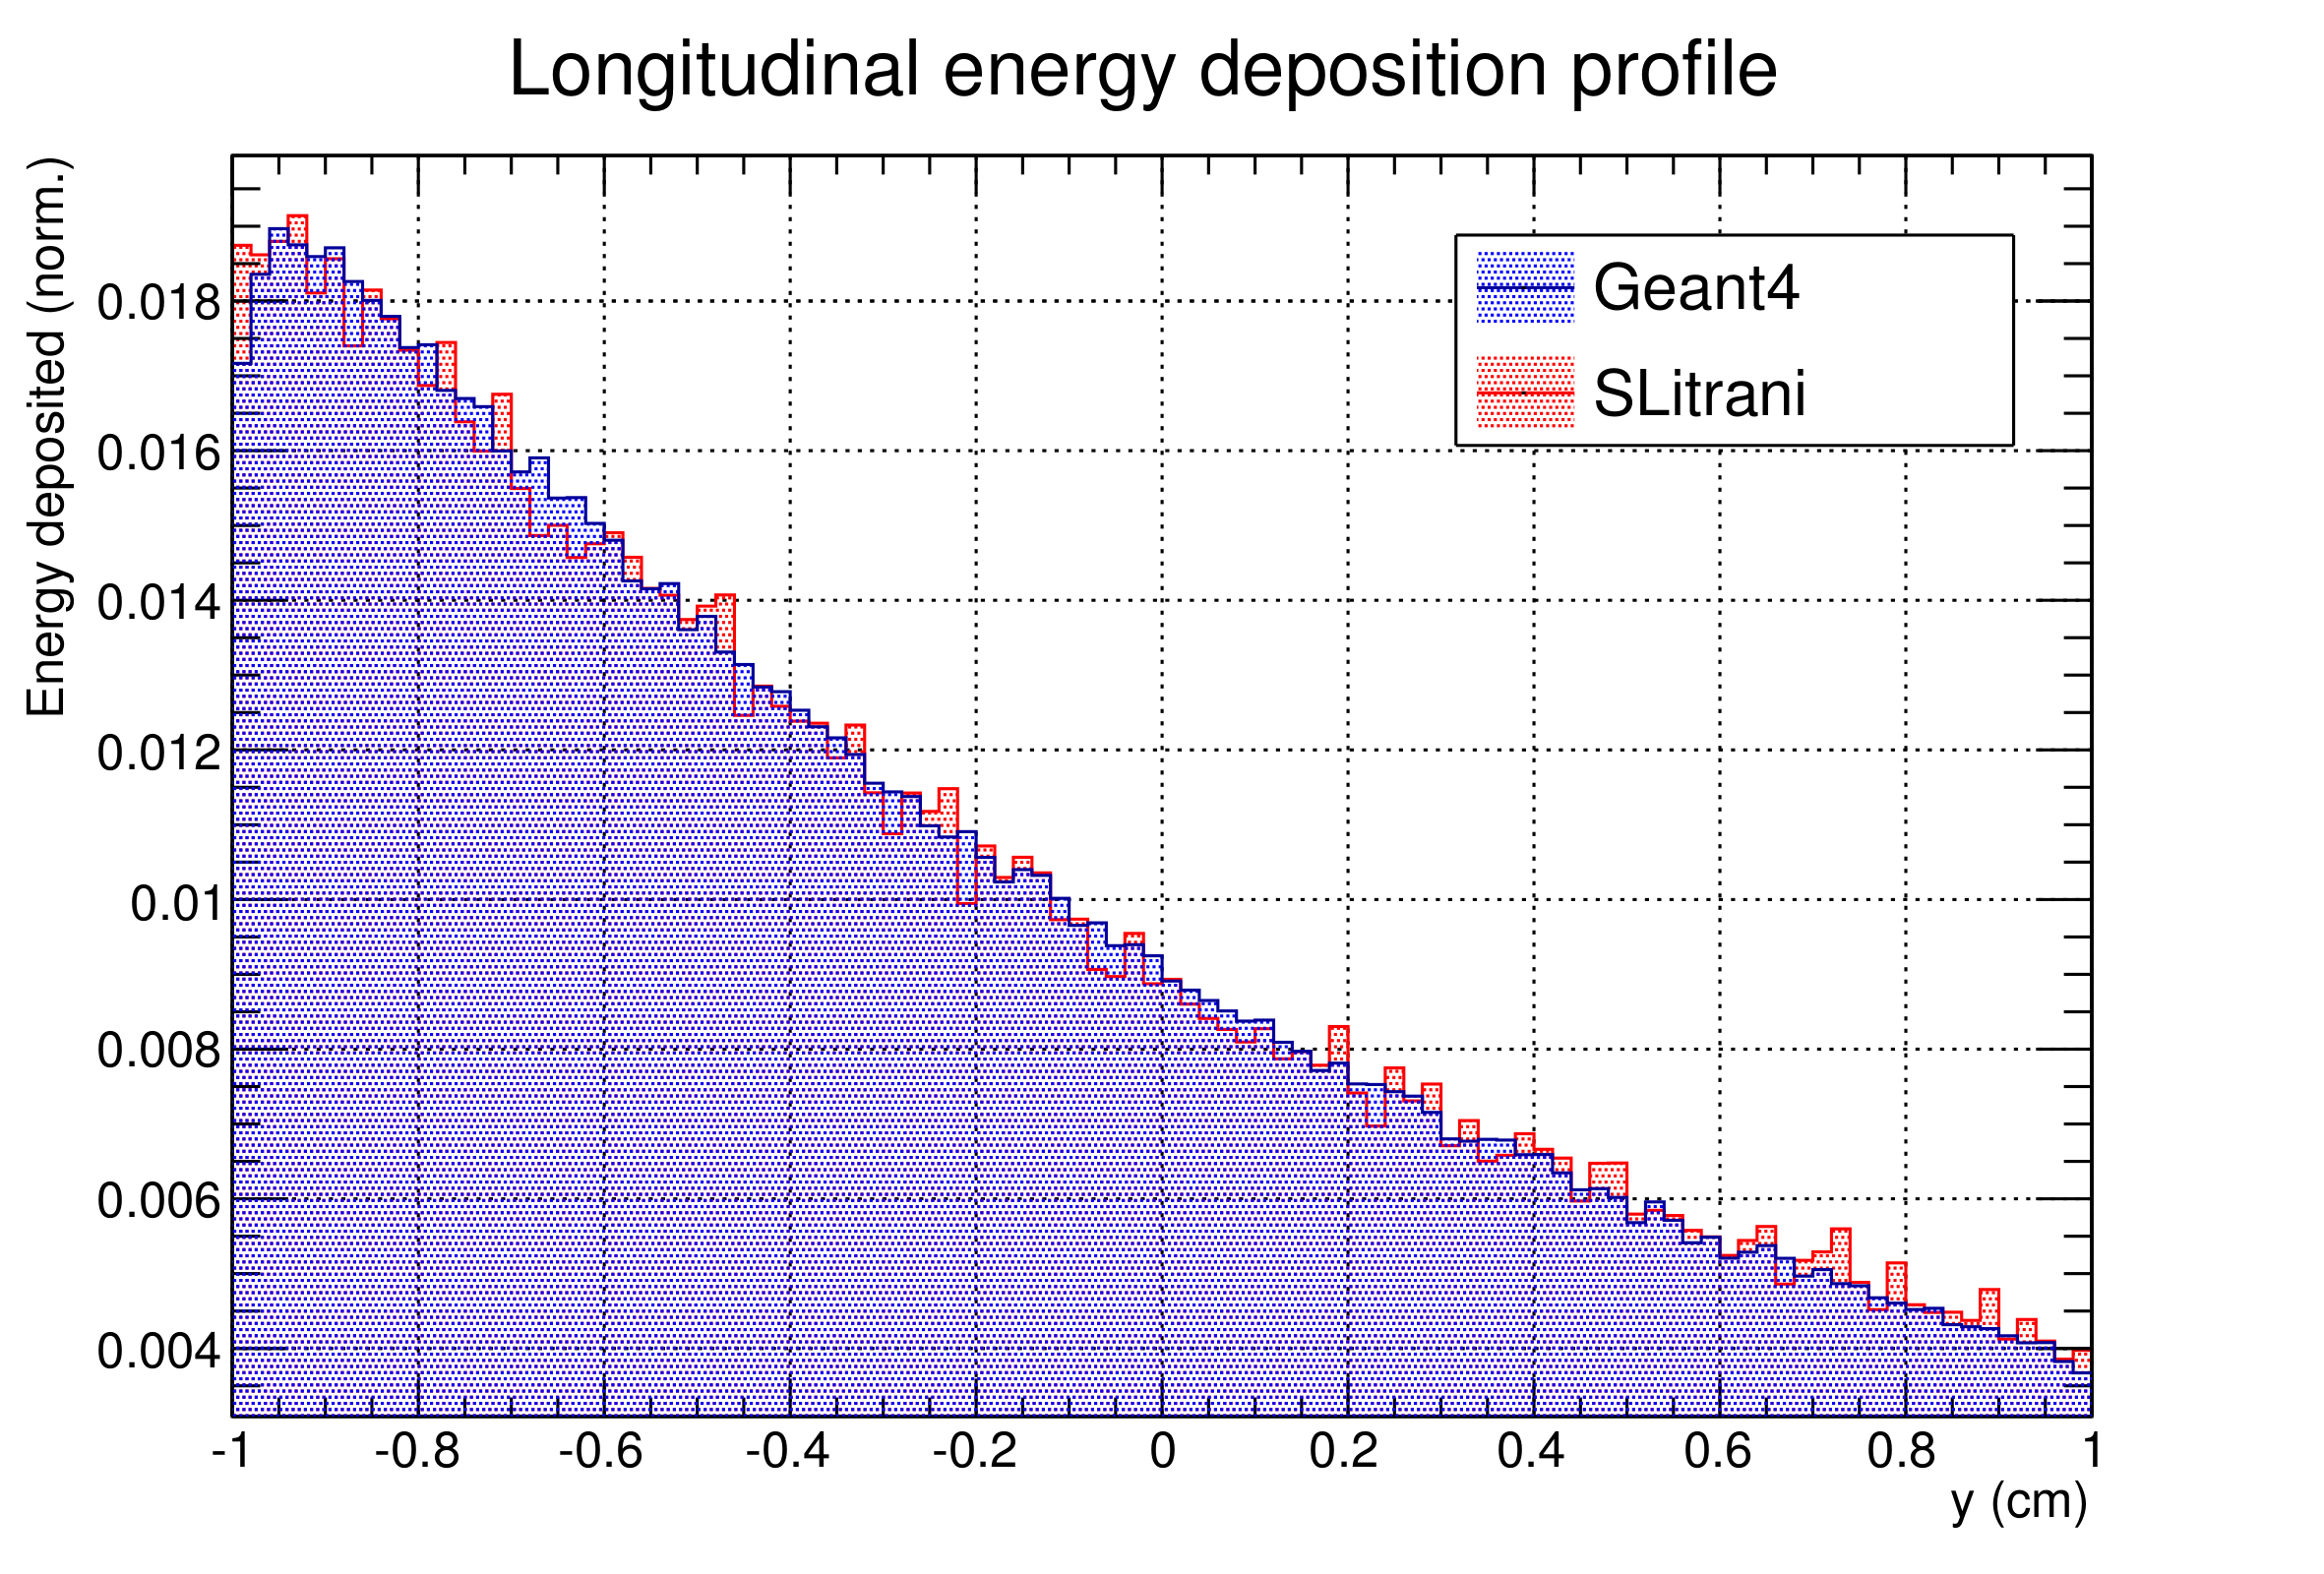
\includegraphics[width=6cm]{../Pictures/Chapter_5/energy_dep.png}
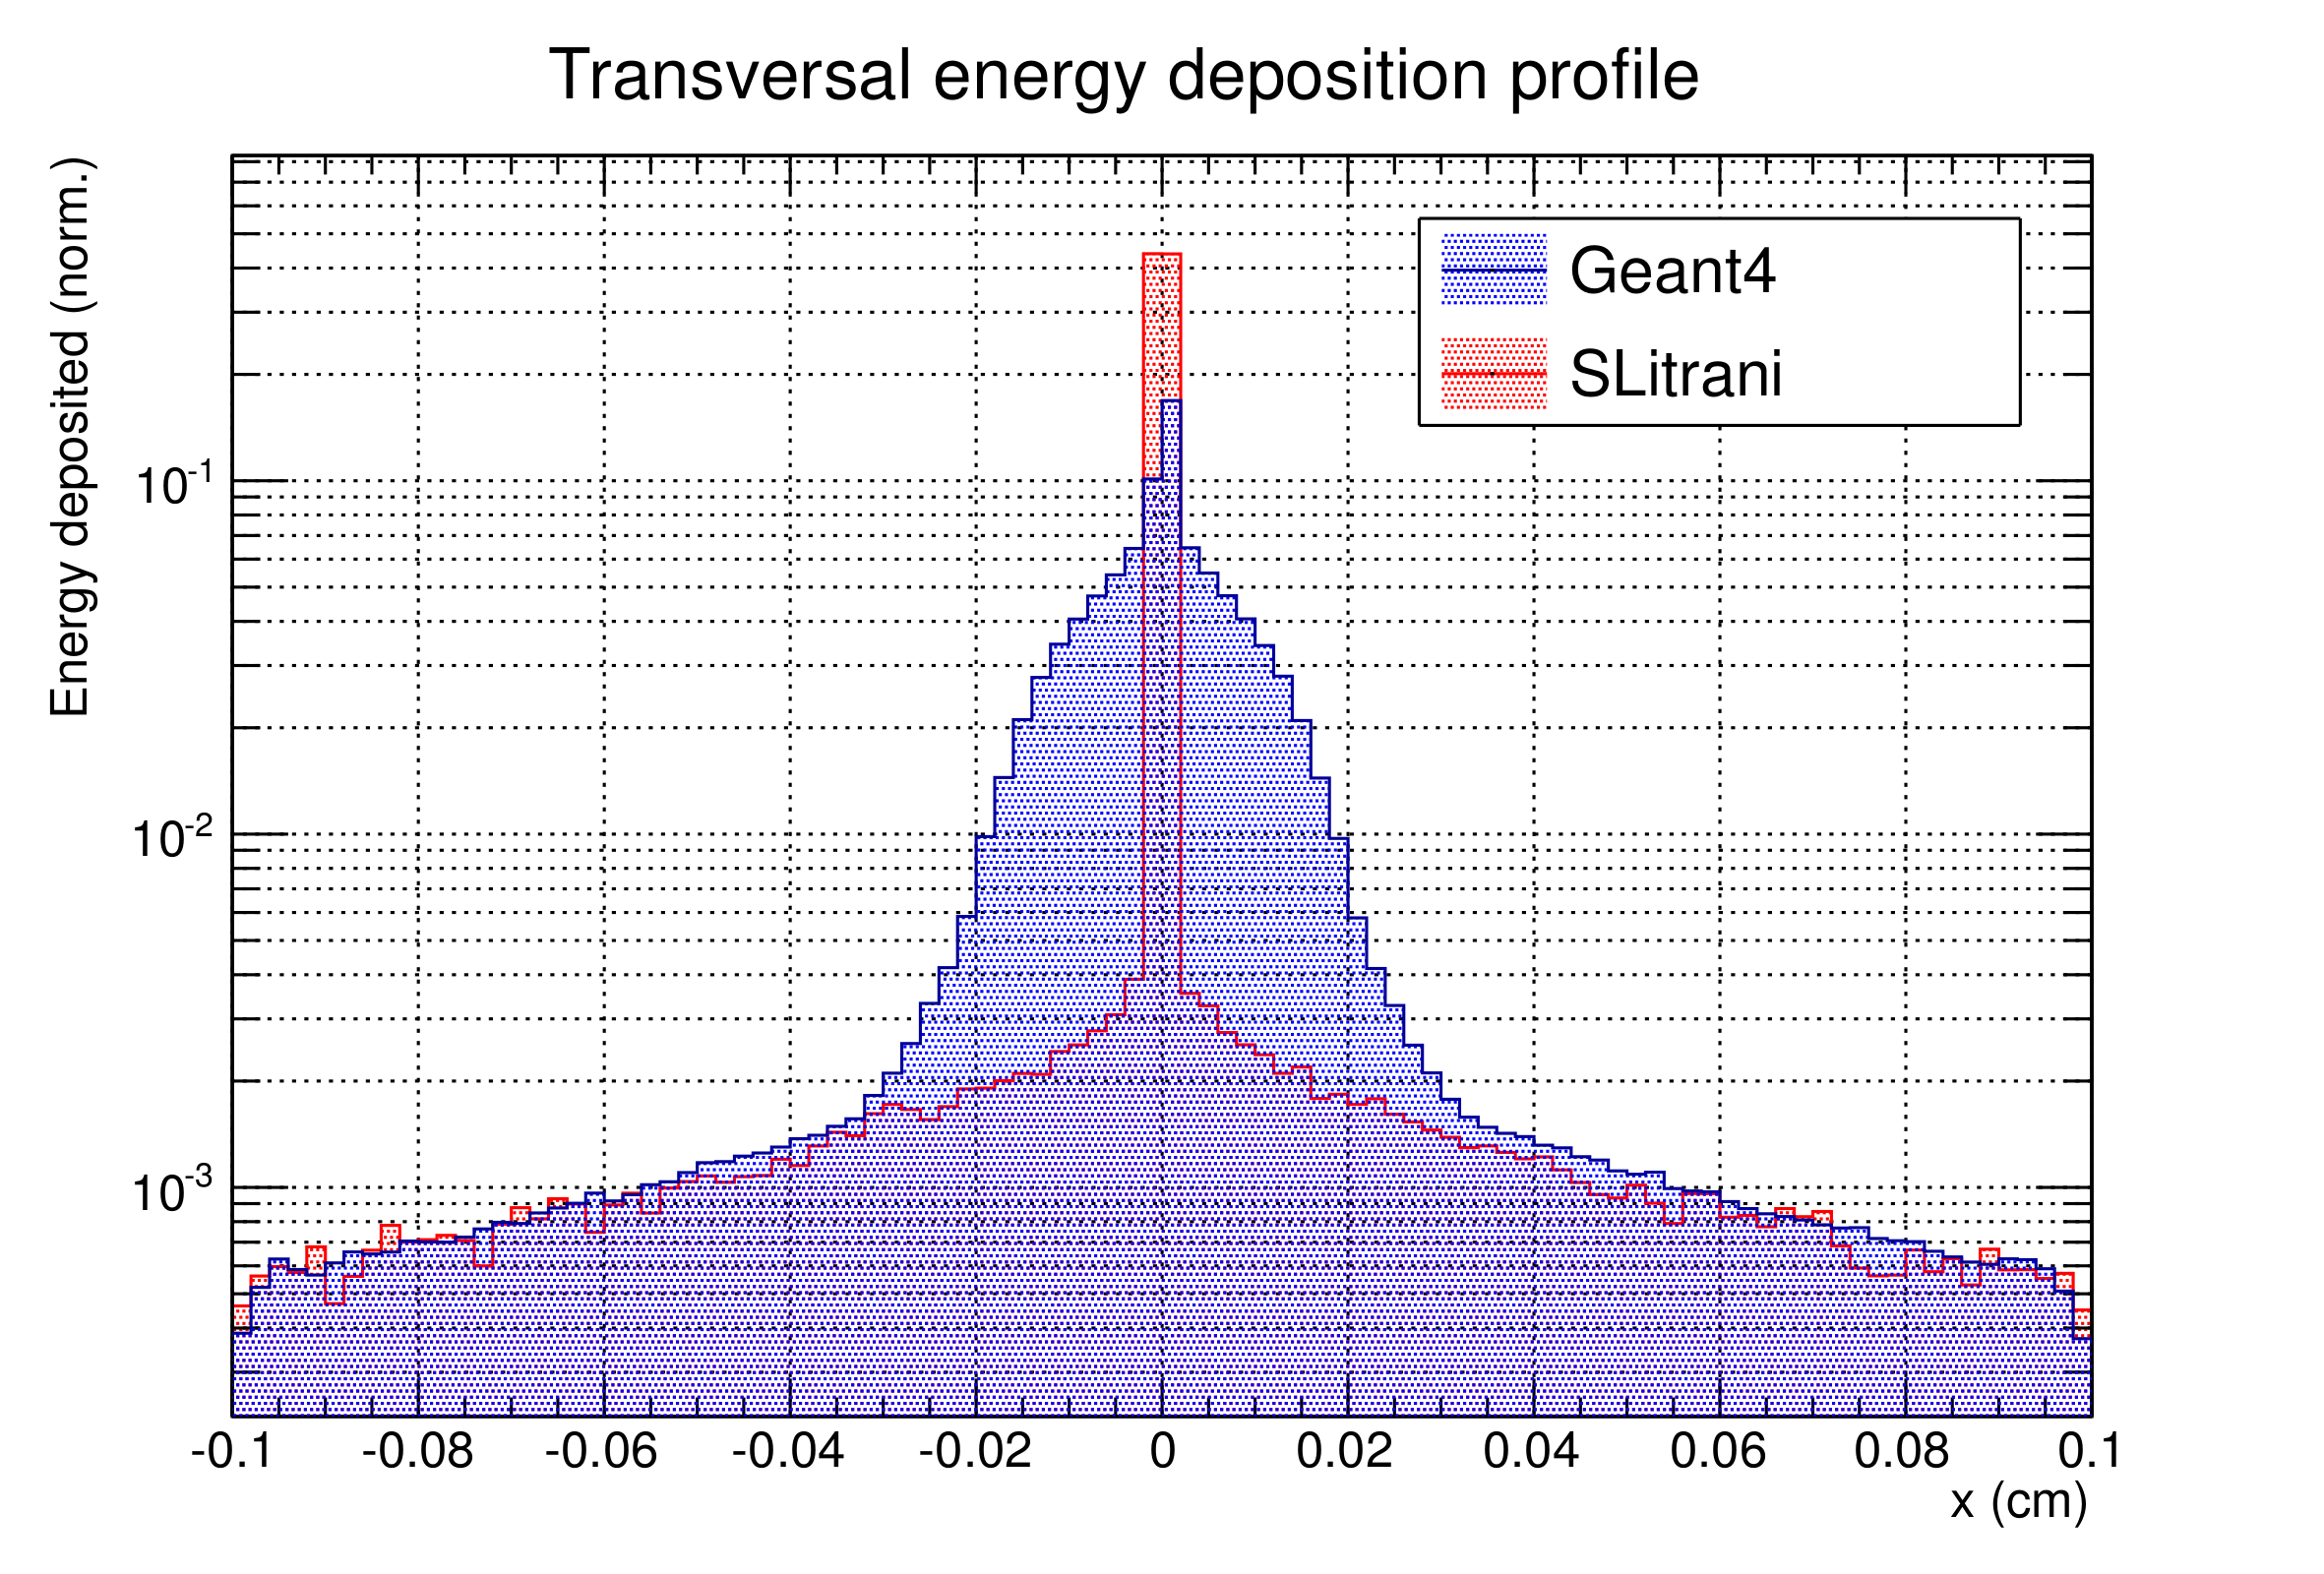
\includegraphics[width=6cm]{../Pictures/Chapter_5/energy_dep_lat.png}
\end{center}
\caption[RMS comparison]{Comparison between energy deposition maps in SLitrani and Geant4 (longitudinal and transversal)}
\label{fig:rms}
\end{figure}
Giving the fact that typical values for light yield of heavy scintillating crystals are around a few tens of thousands photons per MeV, the smearing effect of energy deposition can often be neglected. The same goes for the small amount of Cerenkov photons produced with respect to the number of photons extracted and the subsequent resolution effect.

Nonetheless, as already discussed in the previous chapter, a small but significant impact can be found as soon as timing properties of crystals are taken into account.
\subsection{Cerenkov photons for low energy excitation}
The direction of the Cerenkov photons produced can be neglected, and it retains no value, since the information is completely washed out by the typical path of a low energy electron in the crystalline lattice.
As shown in figure \ref{fig:electron} the path of the electron is tortuous due to the large cross section for multi scattering processes.
\begin{figure}[htbp]
\begin{center}
%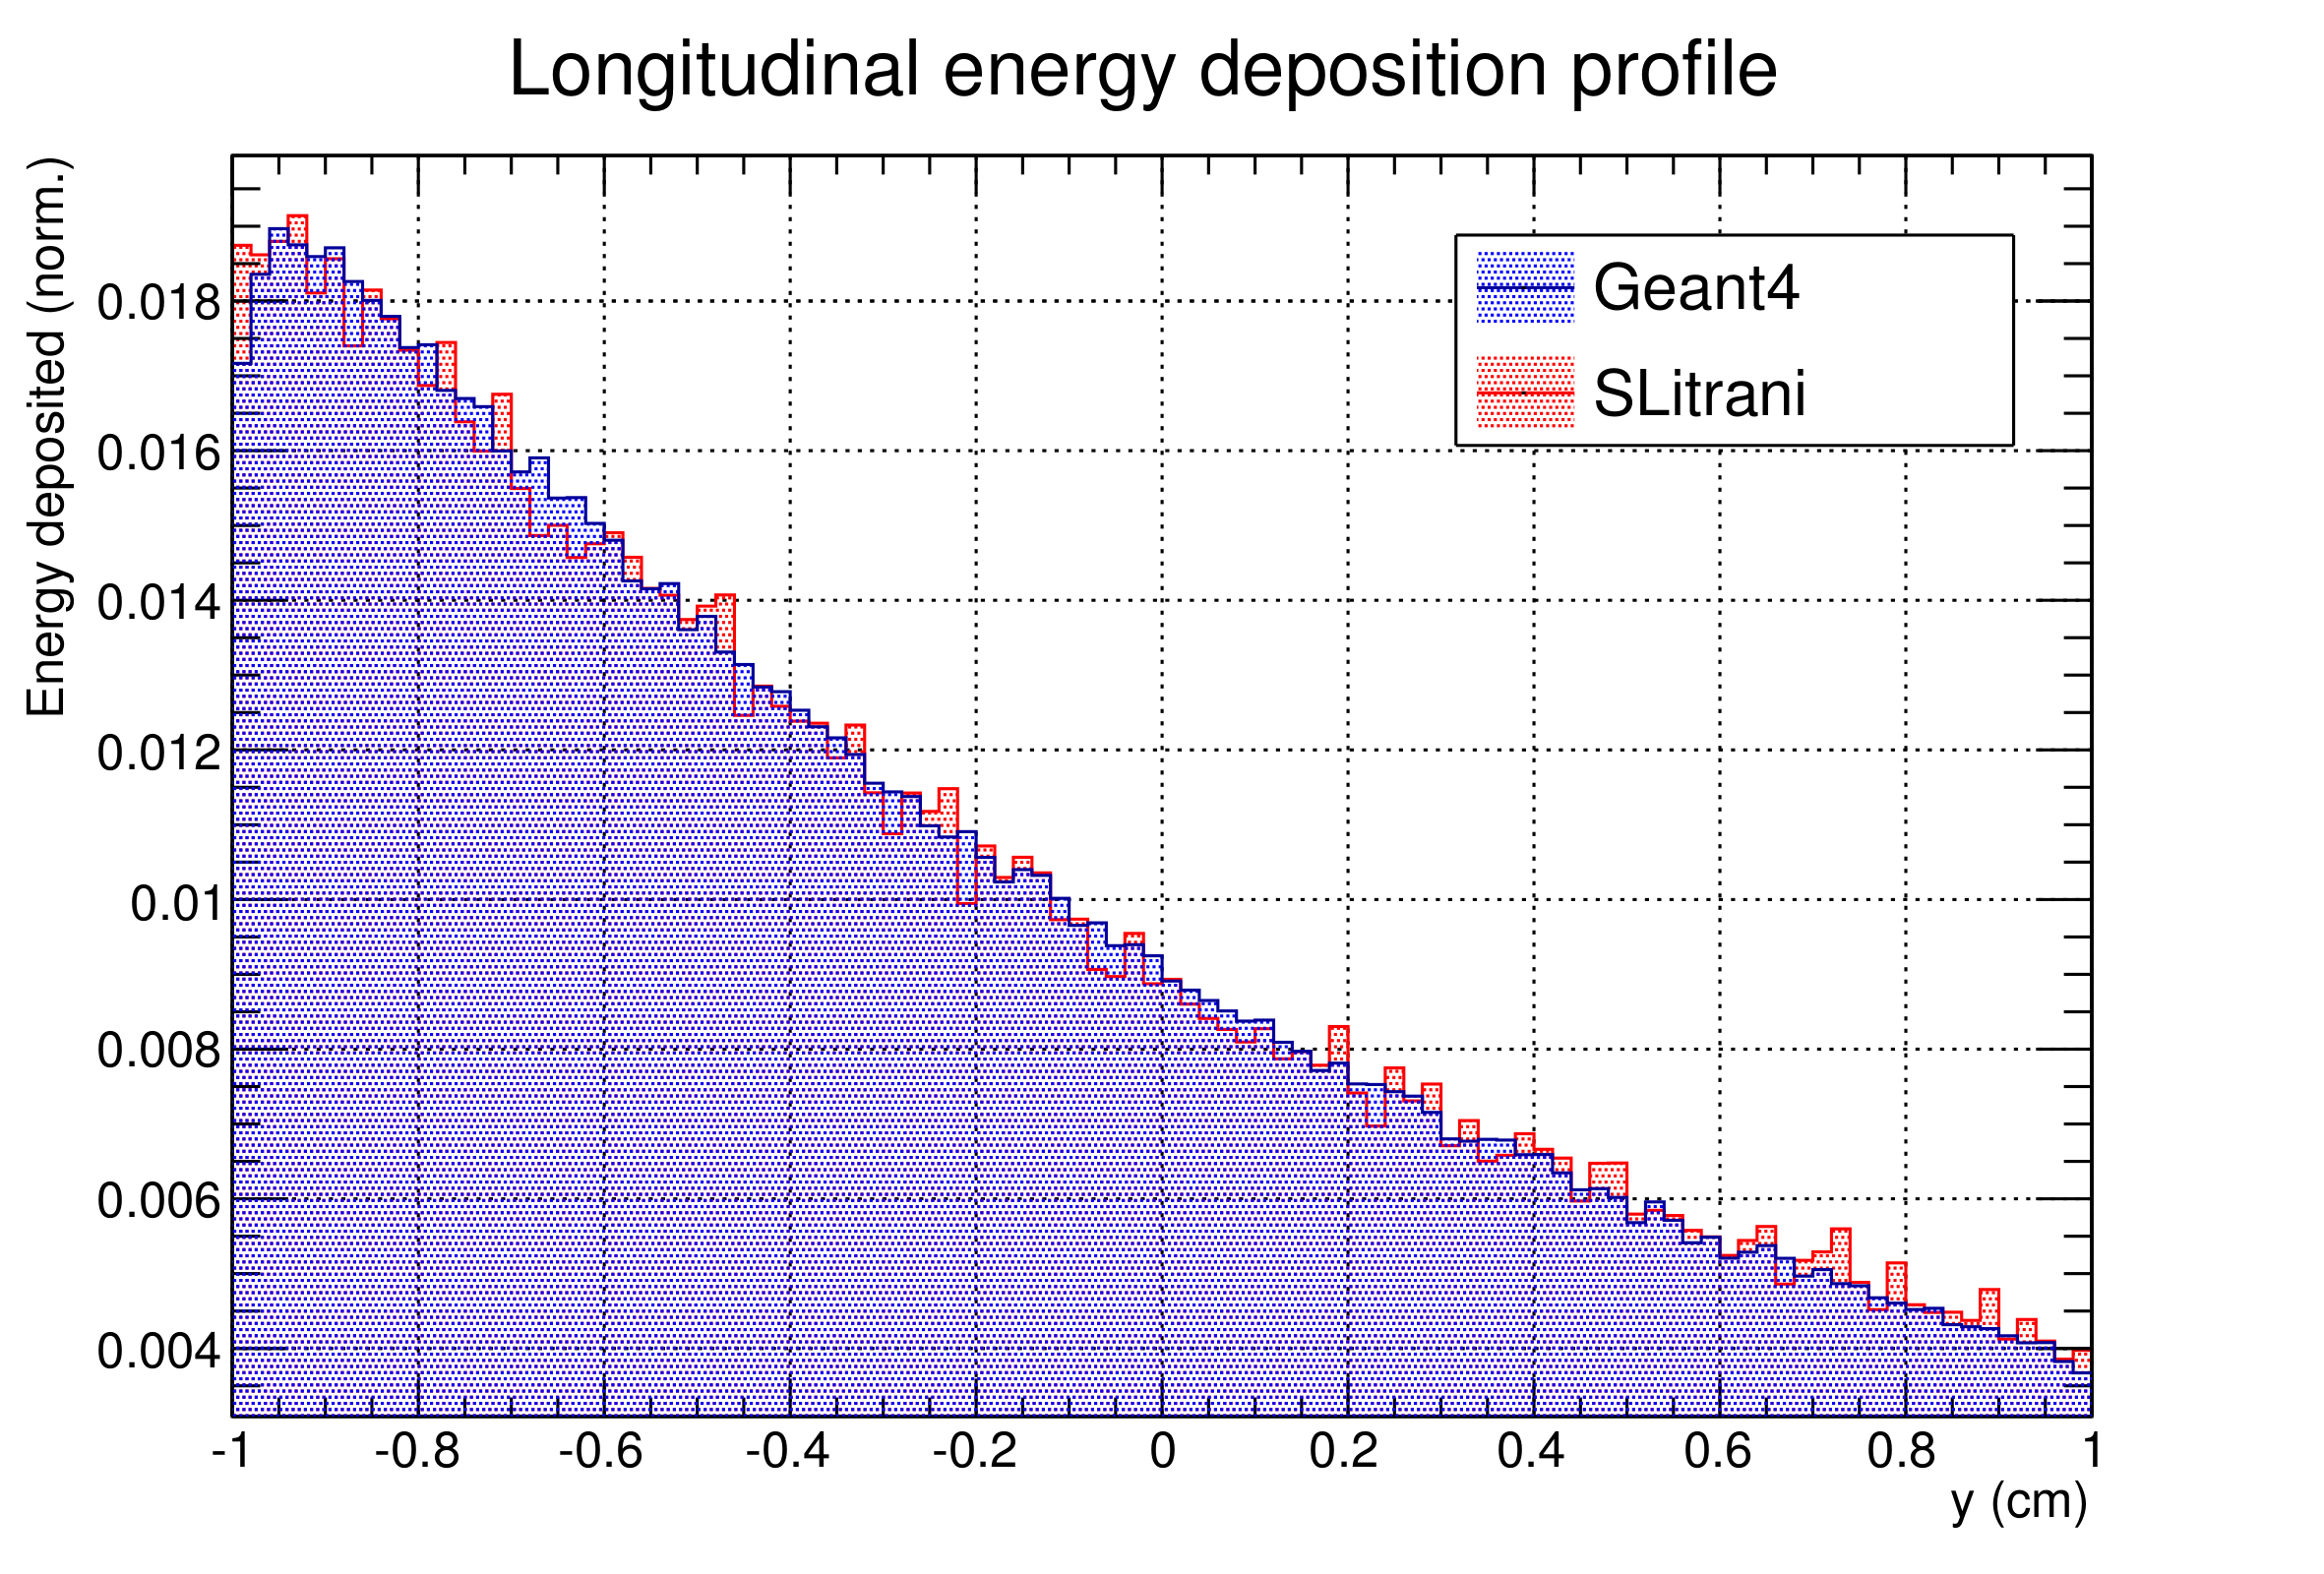
\includegraphics[width=6cm]{../Pictures/Chapter_5/energy_dep.png}
%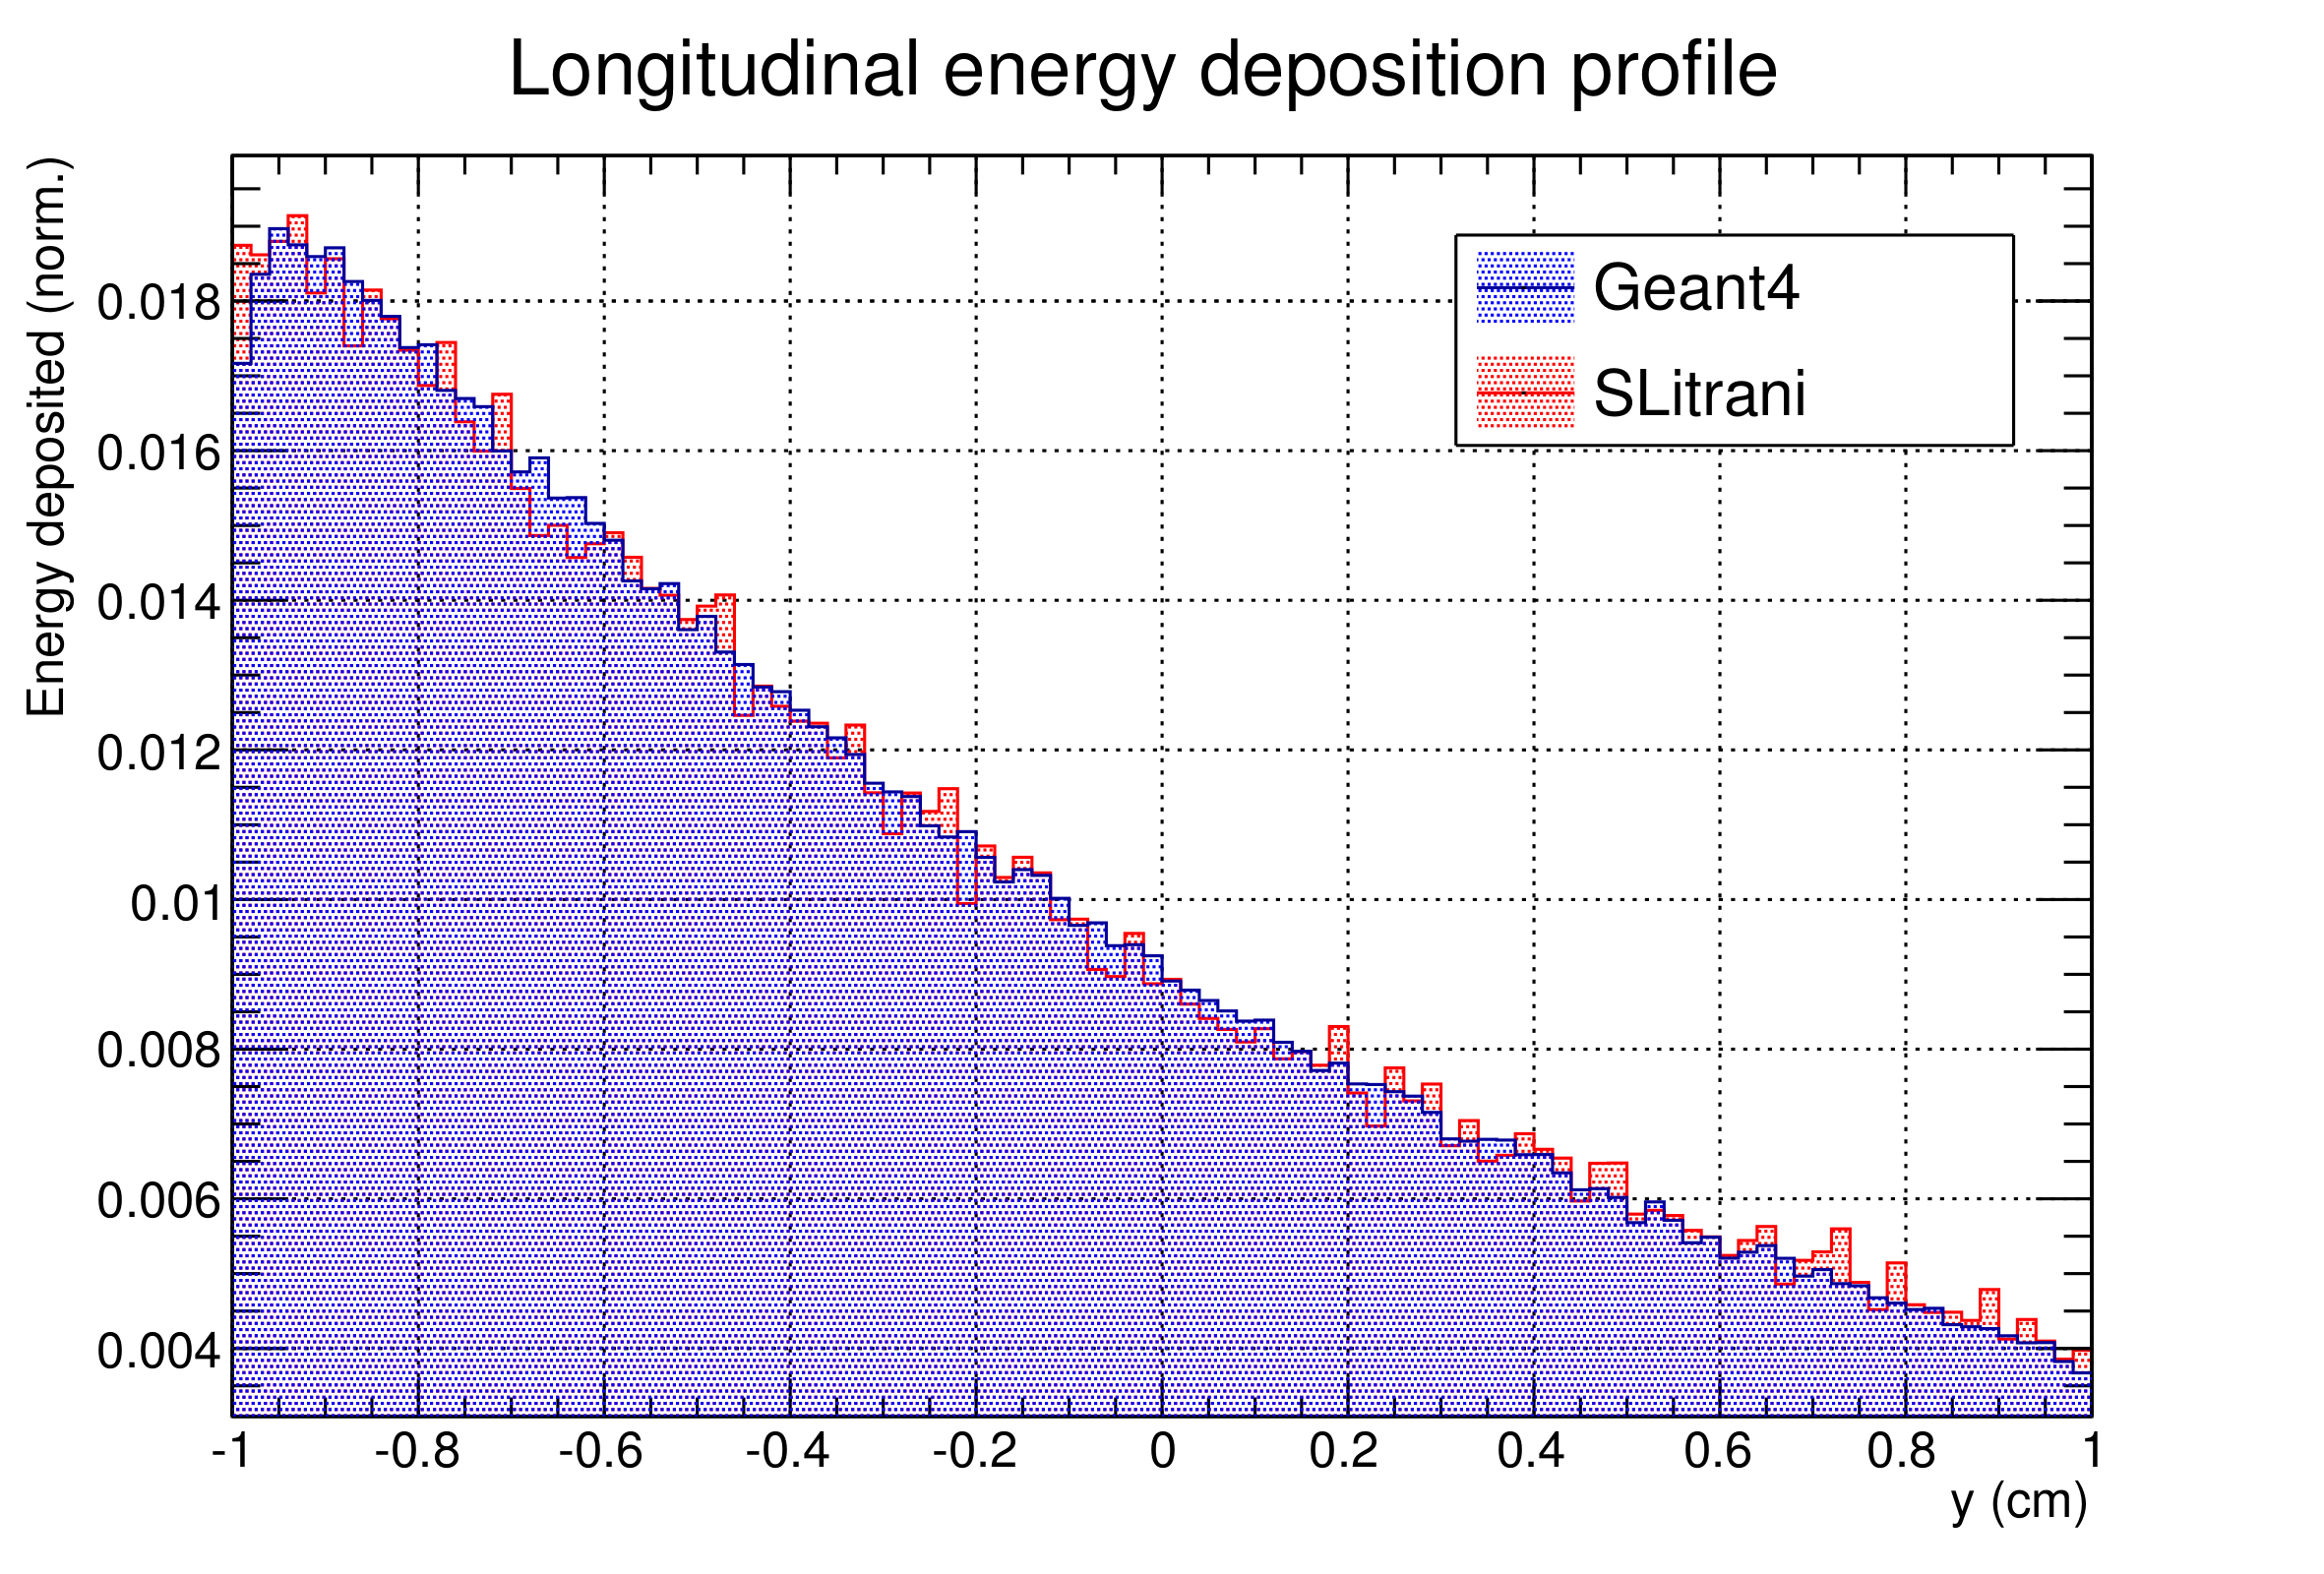
\includegraphics[width=6cm]{../Pictures/Chapter_5/energy_dep.png}
\end{center}
\caption[Electron path in lattice]{Example of path of electron in a LSO: Ce lattice according to Geant4 libraries}
\label{fig:electron}
\end{figure}
On the other hand the first question to be answered when evaluating the impact of Cerenkov photons on time profiles of crystals concerns the number of photons extracted.
It has been shown in chapter 2 that the number of photons produced for different cristalline spacies may be relevant. 
In order to estimate an order of magnitude for the number of photons collected at the exit window of the detector, a simulation was performed in Geant4 using the low energy Penelope libraries. The setup is a simple 2x2x3 mm$^{3}$ crystal hit by a 511 KeV $\gamma$ particle. At this stage, the condition were kept as simple as possible, thus including only Fresnel processes and absorption: the crystal is not wrapped and surrounded by air, the coupling medium to the photo detector is air.

\begin{figure}[htbp]
\begin{center}
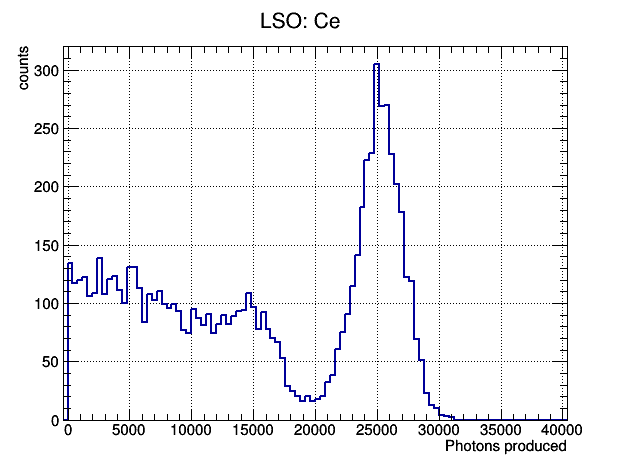
\includegraphics[width=6cm]{../Pictures/Chapter_5/spctrum_LSO.png}
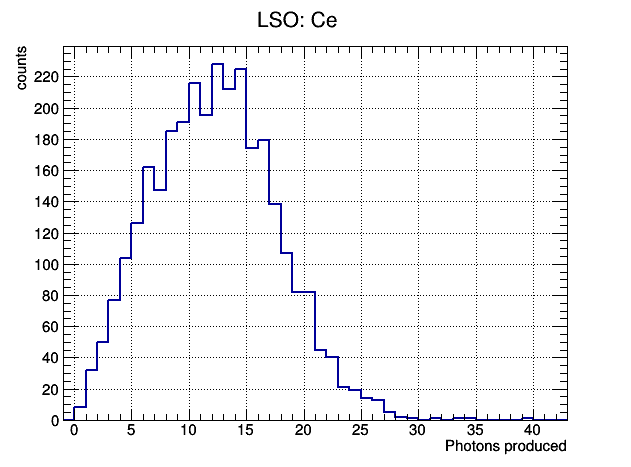
\includegraphics[width=6cm]{../Pictures/Chapter_5/cerenkov_LSO.png}
\end{center}
\caption[]{}
\label{fig:ceren_phot}
\end{figure}
As shown in figure \ref{fig:ceren_phot}, the number of Cerenkov photons, which dependes essentially on the density and refractive index of the medium is in substantial agreement with the theoretical calculation, provided the statistical spread.
A good deal of attention should be posed on the fact that this photons are, at the moment, produced, in the range of the scattered electron. 
The number of photons coupled out is substantially reduced by three factors: 
\begin{itemize}
\item the reduced cone of extraction due to the matching of refractive indices (air-crystal)
\item the transmission curve of the crystal
\item the quantum efficiency of the photo detector
\end{itemize}
For what concerns the refractive indices of the materials simulated, values were taken from \cite{Auffray2009}, \cite{Kuwano2004}, \cite{jellison2012}.
The quantum efficiency influences selectively the the photons extracted, thus influencing the ratio between scintillation and Cerenkov photons. Indeed a photo detector more efficient in the UV would collect a higher number of Cerenkov photons. For this preliminary result a standard photo cathode quantum efficiency has been considered, between 200 and 1000 nm.
Finally the transmission curve allows only certain wavelengths to be transmitted due to the absoprtion by the luminescence centers of the crystal. The values used have been measured for samples on the crystalline species used with the method outlined in the next sections.

\begin{table}[h]
\begin{center}
\begin{tabular}{llll}
Crystal  & Calculated & Produced & Collected \\
LSO: Ce  & 15         & 12.1     & 1.4       \\
PbWO4    & 21         & 18       & 4.1       \\
LuAG: Ce & 25         & 20       & 6         \\
CeF3     &            &          &           \\
BGO      & 23         & 25       & 3.2      
\end{tabular}
\end{center}
\caption[Cerenkov photons]{Example of Cerenkov photons calculated and simulated (produced and collected) for different crystalline species}
\label{table:cer}
\end{table}

As already said this small number can be neglected in most cases: as shown in the previous chapter their role becomes less and less relevant as the time constants of the crystal get fast. For main  scintillators photons produced and collected are shown in table \ref{table:cer}. This is in agreement with previous studies, such as \cite{Brunner2014}.

In particular they are negligible when the ratio between Cerenkov photons collected and scintillation photons collected becomes low. In this case most of the photons collected come from a scintillation event.
When dealing with PET like setups one should also take into account the fact that selection on the photopeak usually is mandatory for improving the signal to noise ratio. This changes also the ratio between Cerenkov and scintillation photons, since it is muche more likely for a event with a photoelectric effect to couple out a Cerenkov photon. In the analysis run in the last chapters this will not be completely true since no selection will take place.

\begin{figure}[htbp]
\begin{center}
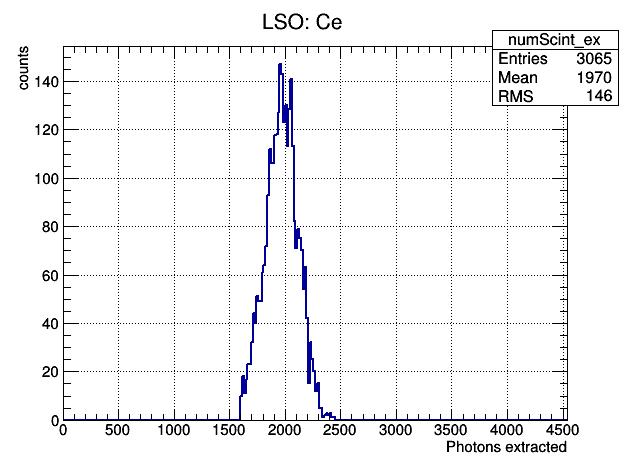
\includegraphics[width=6cm]{../Pictures/Chapter_5/pp_LSO.png}
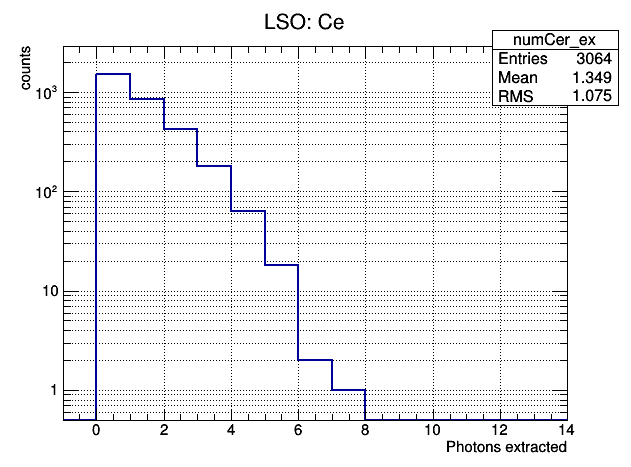
\includegraphics[width=6cm]{../Pictures/Chapter_5/cer_extr_LSO.png}
\end{center}
\caption[Photopeak selection for Cerenkov simulation]{The spectrum is selected on the LSO photo peak (left) and the number of Cerenkov collected changes slightly (right)}
\label{fig:ceren_pp}
\end{figure}
As a final remark it is interesting to underline the timing characteristics of the Cerenkov spectrum. Indeed these photons are produced promptly, and as shown in the previous chapter they can influence, albeit slightly, the time resolution. They can especially change the way we set thresholds on events.
%qui serve la roba sui fotoni negli slot temporali
As shown in figure \ref{fig:time_ratio} in the first 100 ps a relevant part of the photons collected is taken by scintillation photons. This means that they can not be completely neglected, as emerged in the previous chapter.
\begin{figure}[htbp]
\begin{center}
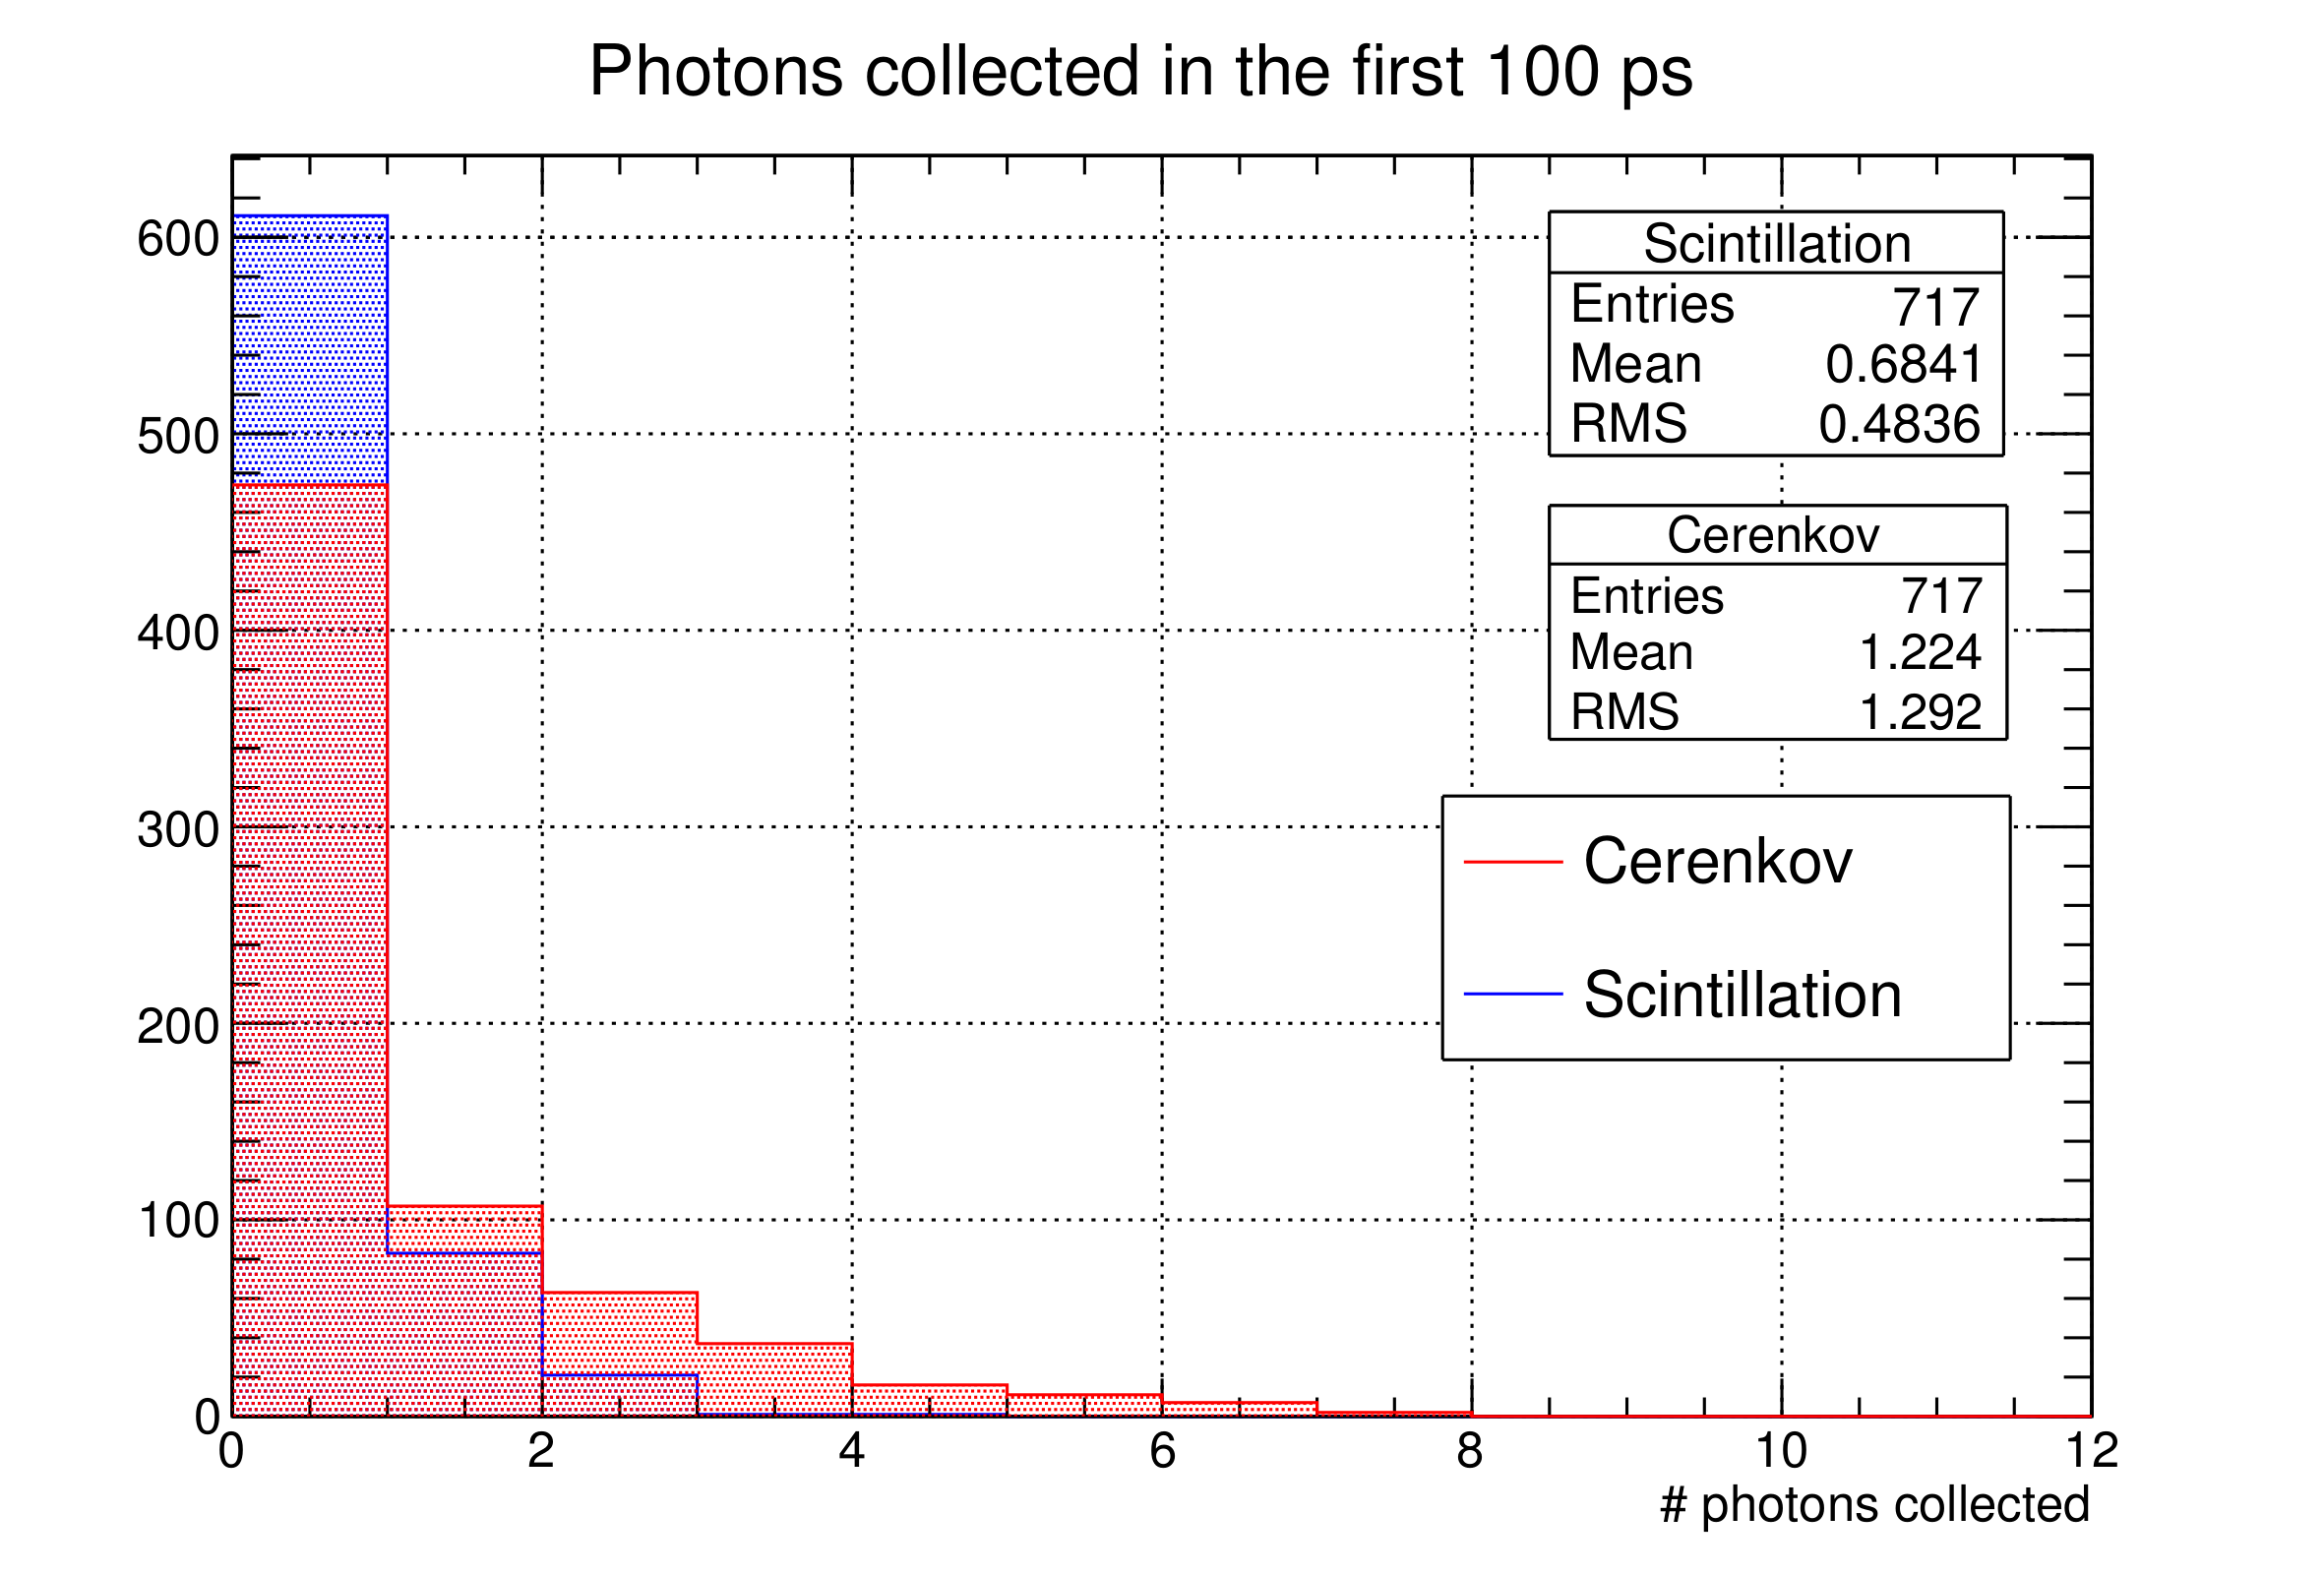
\includegraphics[width=8cm]{../Pictures/Chapter_5/cer_second_balance.png}
\end{center}
\caption[Scintillation/Cerenkov ratio in the first 100 ps]{The Cerenkov photons collected in the first 100 ps are comparable to the scintillation collection.}
\label{fig:time_ratio}
\end{figure}

\subsection{Rise time model}
The rise time model implemented in Geant4 is very simple, and given the energy depoistion map in the crystal volume very similar to that of SLitrani. 
As soon as the program calls for energy deposition in a specific point, below the cut value set for the simulation, the scintillation process is called. 
At this point a bunch of isotropically distributed photons is produced, with the time profiles specified for the material.
All the parameters are defined at input: light yield (photons per MeV), energy resolution scale, scattering length, absorption length, index of refraction, fluorescence spectrum. 

In terms of timing, the LiverMore/Penelope libraries allow for reliable tracking until 250 eV. This means that the time scale that divides this level of energy (tens of times higher than the band gap of heavy scintillators) to the recombiantion stage is included in the rise time parameters. Thus there is no model describing thermalization stage, that is all the chain of processes that leads electron hole pairs to recombine at luminescent centers. Attempts to include this stage in a simulation frame have been performed separately, see for example the work presented \cite{Vasiliev2013}.

As a consequence, simulations allow for good modelling of processes taking place above the ionization threshold and until the lower bound of multiscattering processes in low energy electromagnetic libraries. Moreover, as soon as the production of photons takes place with the parameters plugged in for the specific material in use, photons are tracked according to the optical characteristics of the material.

This happens for the two software packages, but SLitrani does not account for Cerenkov events. As shown in figure \ref{fig:scint_cer} this events account for a large part of the rising edge of the signal, thus making Geant4 the ideal choice for simulations concerning timing.
\begin{figure}[htbp]
\begin{center}
%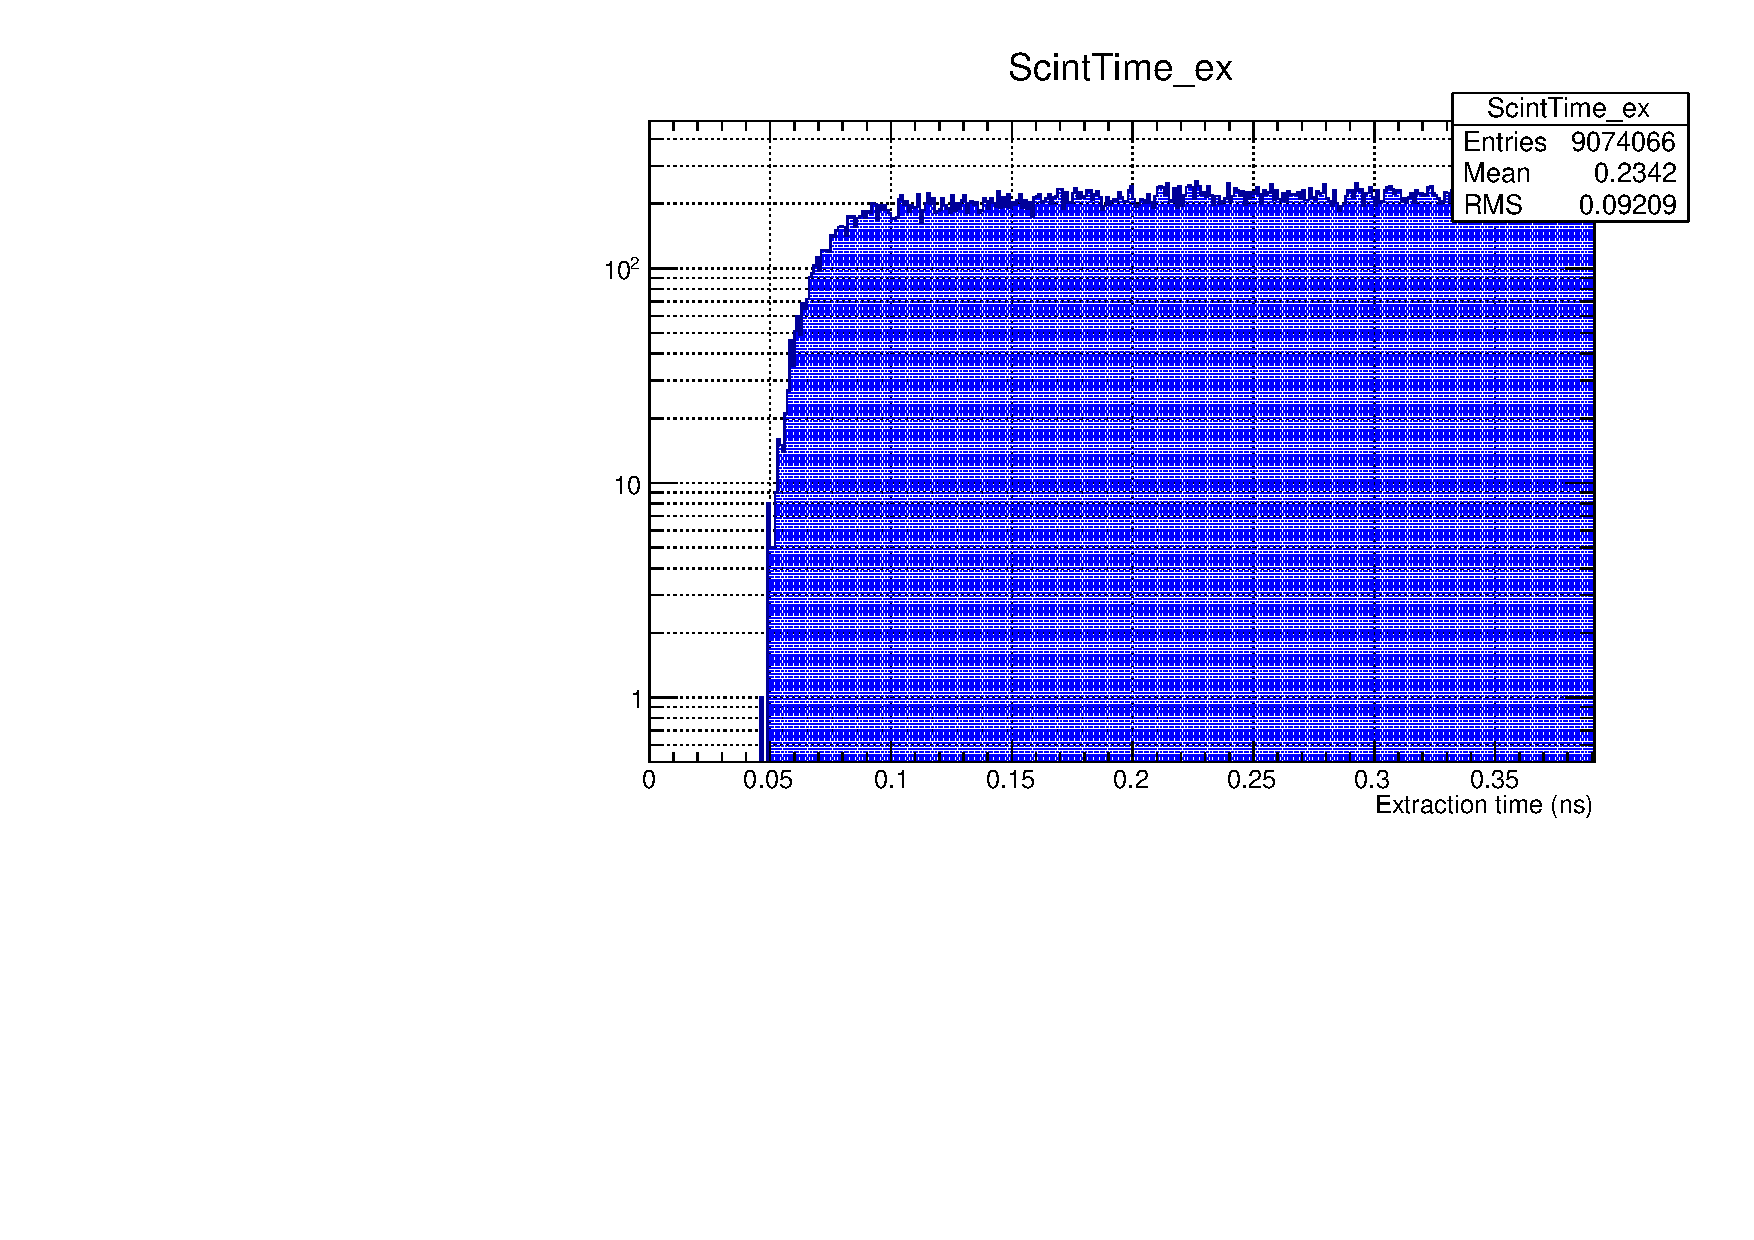
\includegraphics[width=6cm]{../Pictures/Chapter_5/scint_time_ex.pdf}
%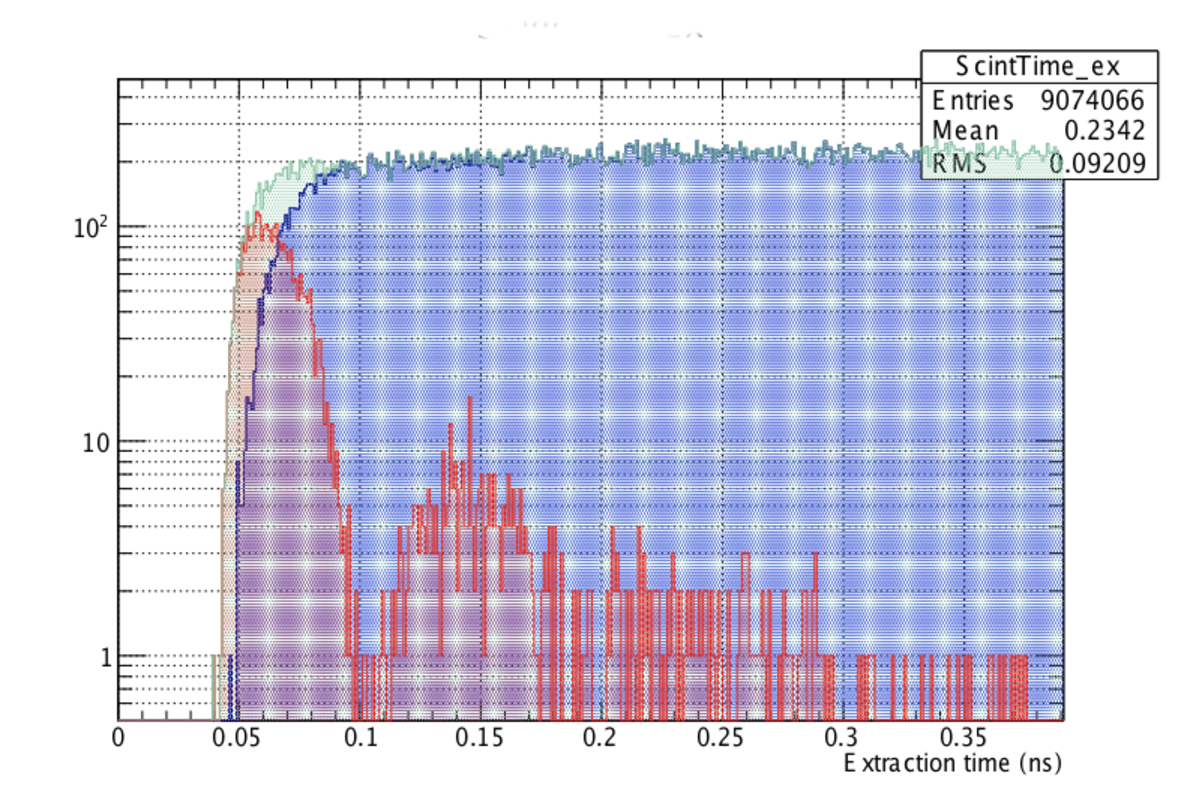
\includegraphics[width=6cm]{../Pictures/Chapter_5/sum_time_ex.pdf}
\end{center}
\caption[Simulated time profiles for LSO]{Simulated time profiles for LSO in SLitrani (left) and Geant4 (right)}
\label{fig:scint_cer}
\end{figure}

\subsection{Absorption and surface treatment}
Optical photons generated inside a crystal may undergo absorption processes (in the bulk or at a surface) and boundary interactions before being extracted or killed.
In order to test the differences between the softwares these events were tested with specified input parameters for absorption length and surface characteristics.
For absorption lenght optical photons were generated by a monochromatic source in the center of a very extended crystal. Reflaction and refraction coefficients, on the other hand, where tested with a monochromatic beam of photons from the center of the crystal towards an interface with air.

The ratio of results obtained in SLitrani and Geant4, for LSO demonstrate perfect agreement between the two Monte Carlo software as shown in figure \ref{fig:abs}, both for Fresnel interaction and absorption processes. The parameters for the simulations were extracted with the procedure described in the next section.
\begin{figure}[htbp]
\begin{center}
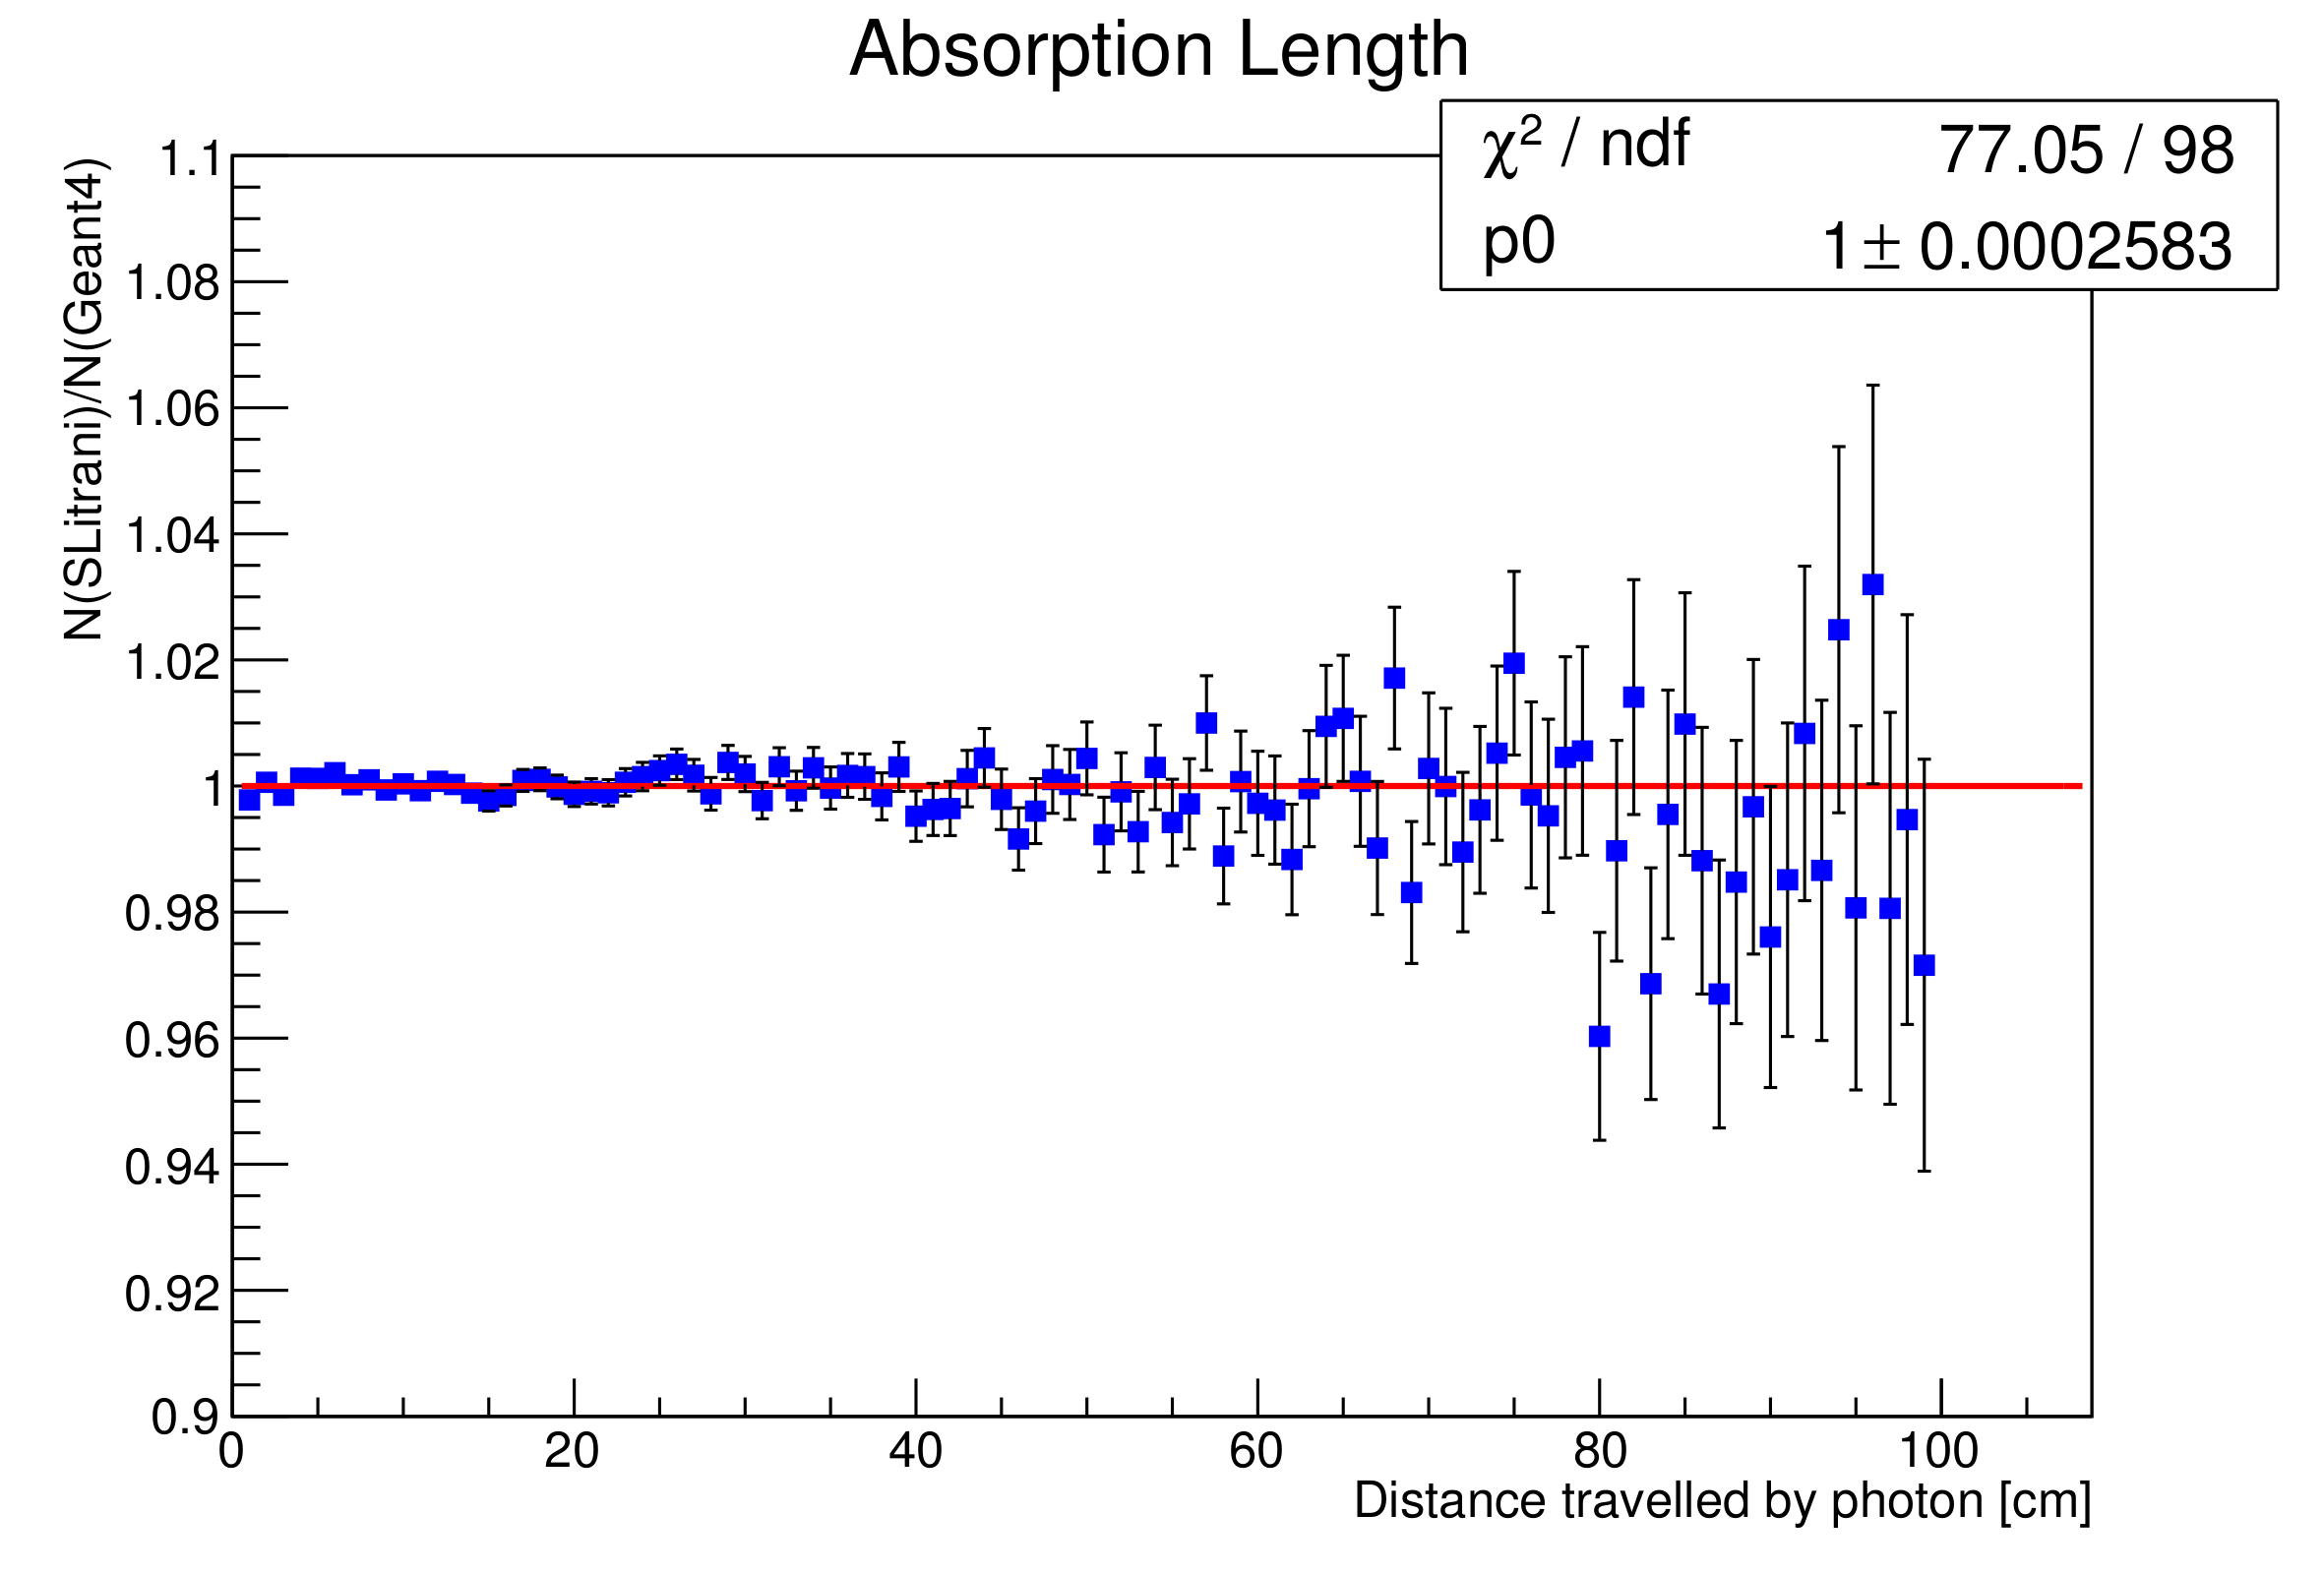
\includegraphics[width=6cm]{../Pictures/Chapter_5/abs.png}
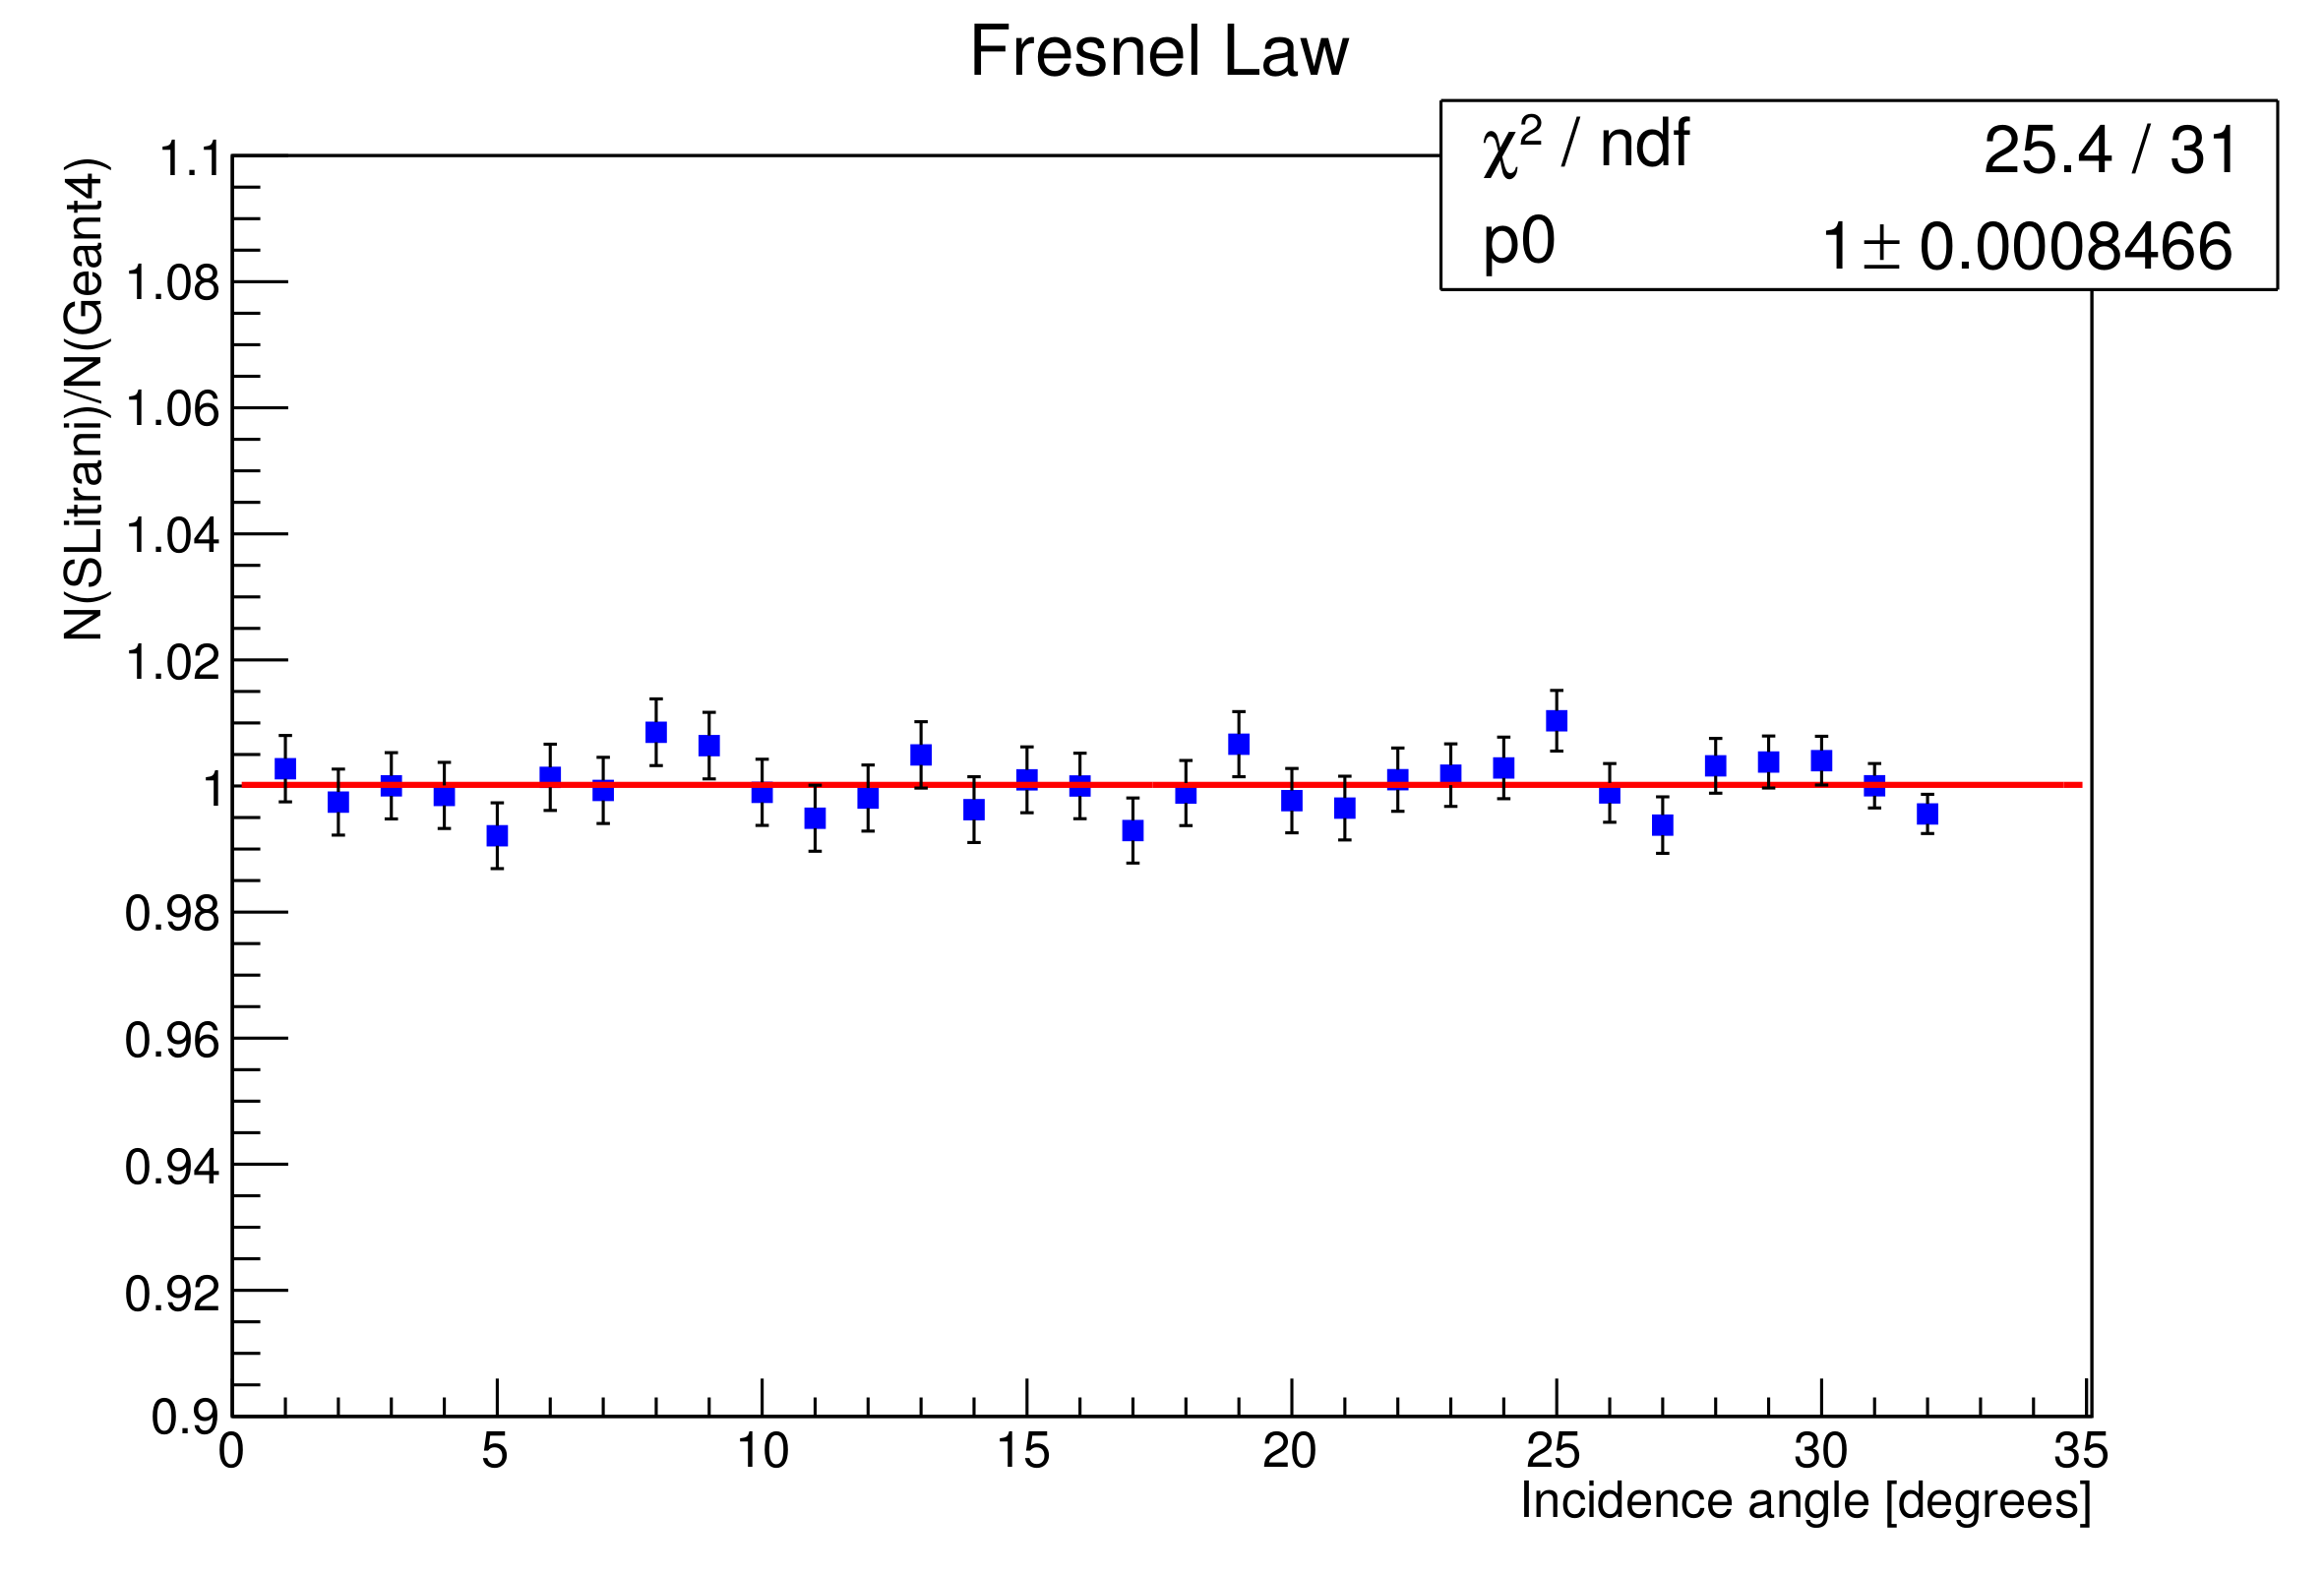
\includegraphics[width=6cm]{../Pictures/Chapter_5/fresnel.png}
\end{center}
\caption[]{}
\label{fig:abs}
\end{figure}

In order to test the models for boundary interaction with wrappings or coatings, the absorption of photons at boundary interface was tested by firing a monochromatic beam of photons towards the surface boundary and varying the incidence angle. The results obtained for the two software are shown in figure \ref{fig:surface}.
A significant difference is found for diffusive wrappings, with SLitrani showing an higher absorption rate for high incidence angles.
\begin{figure}[htbp]
\begin{center}
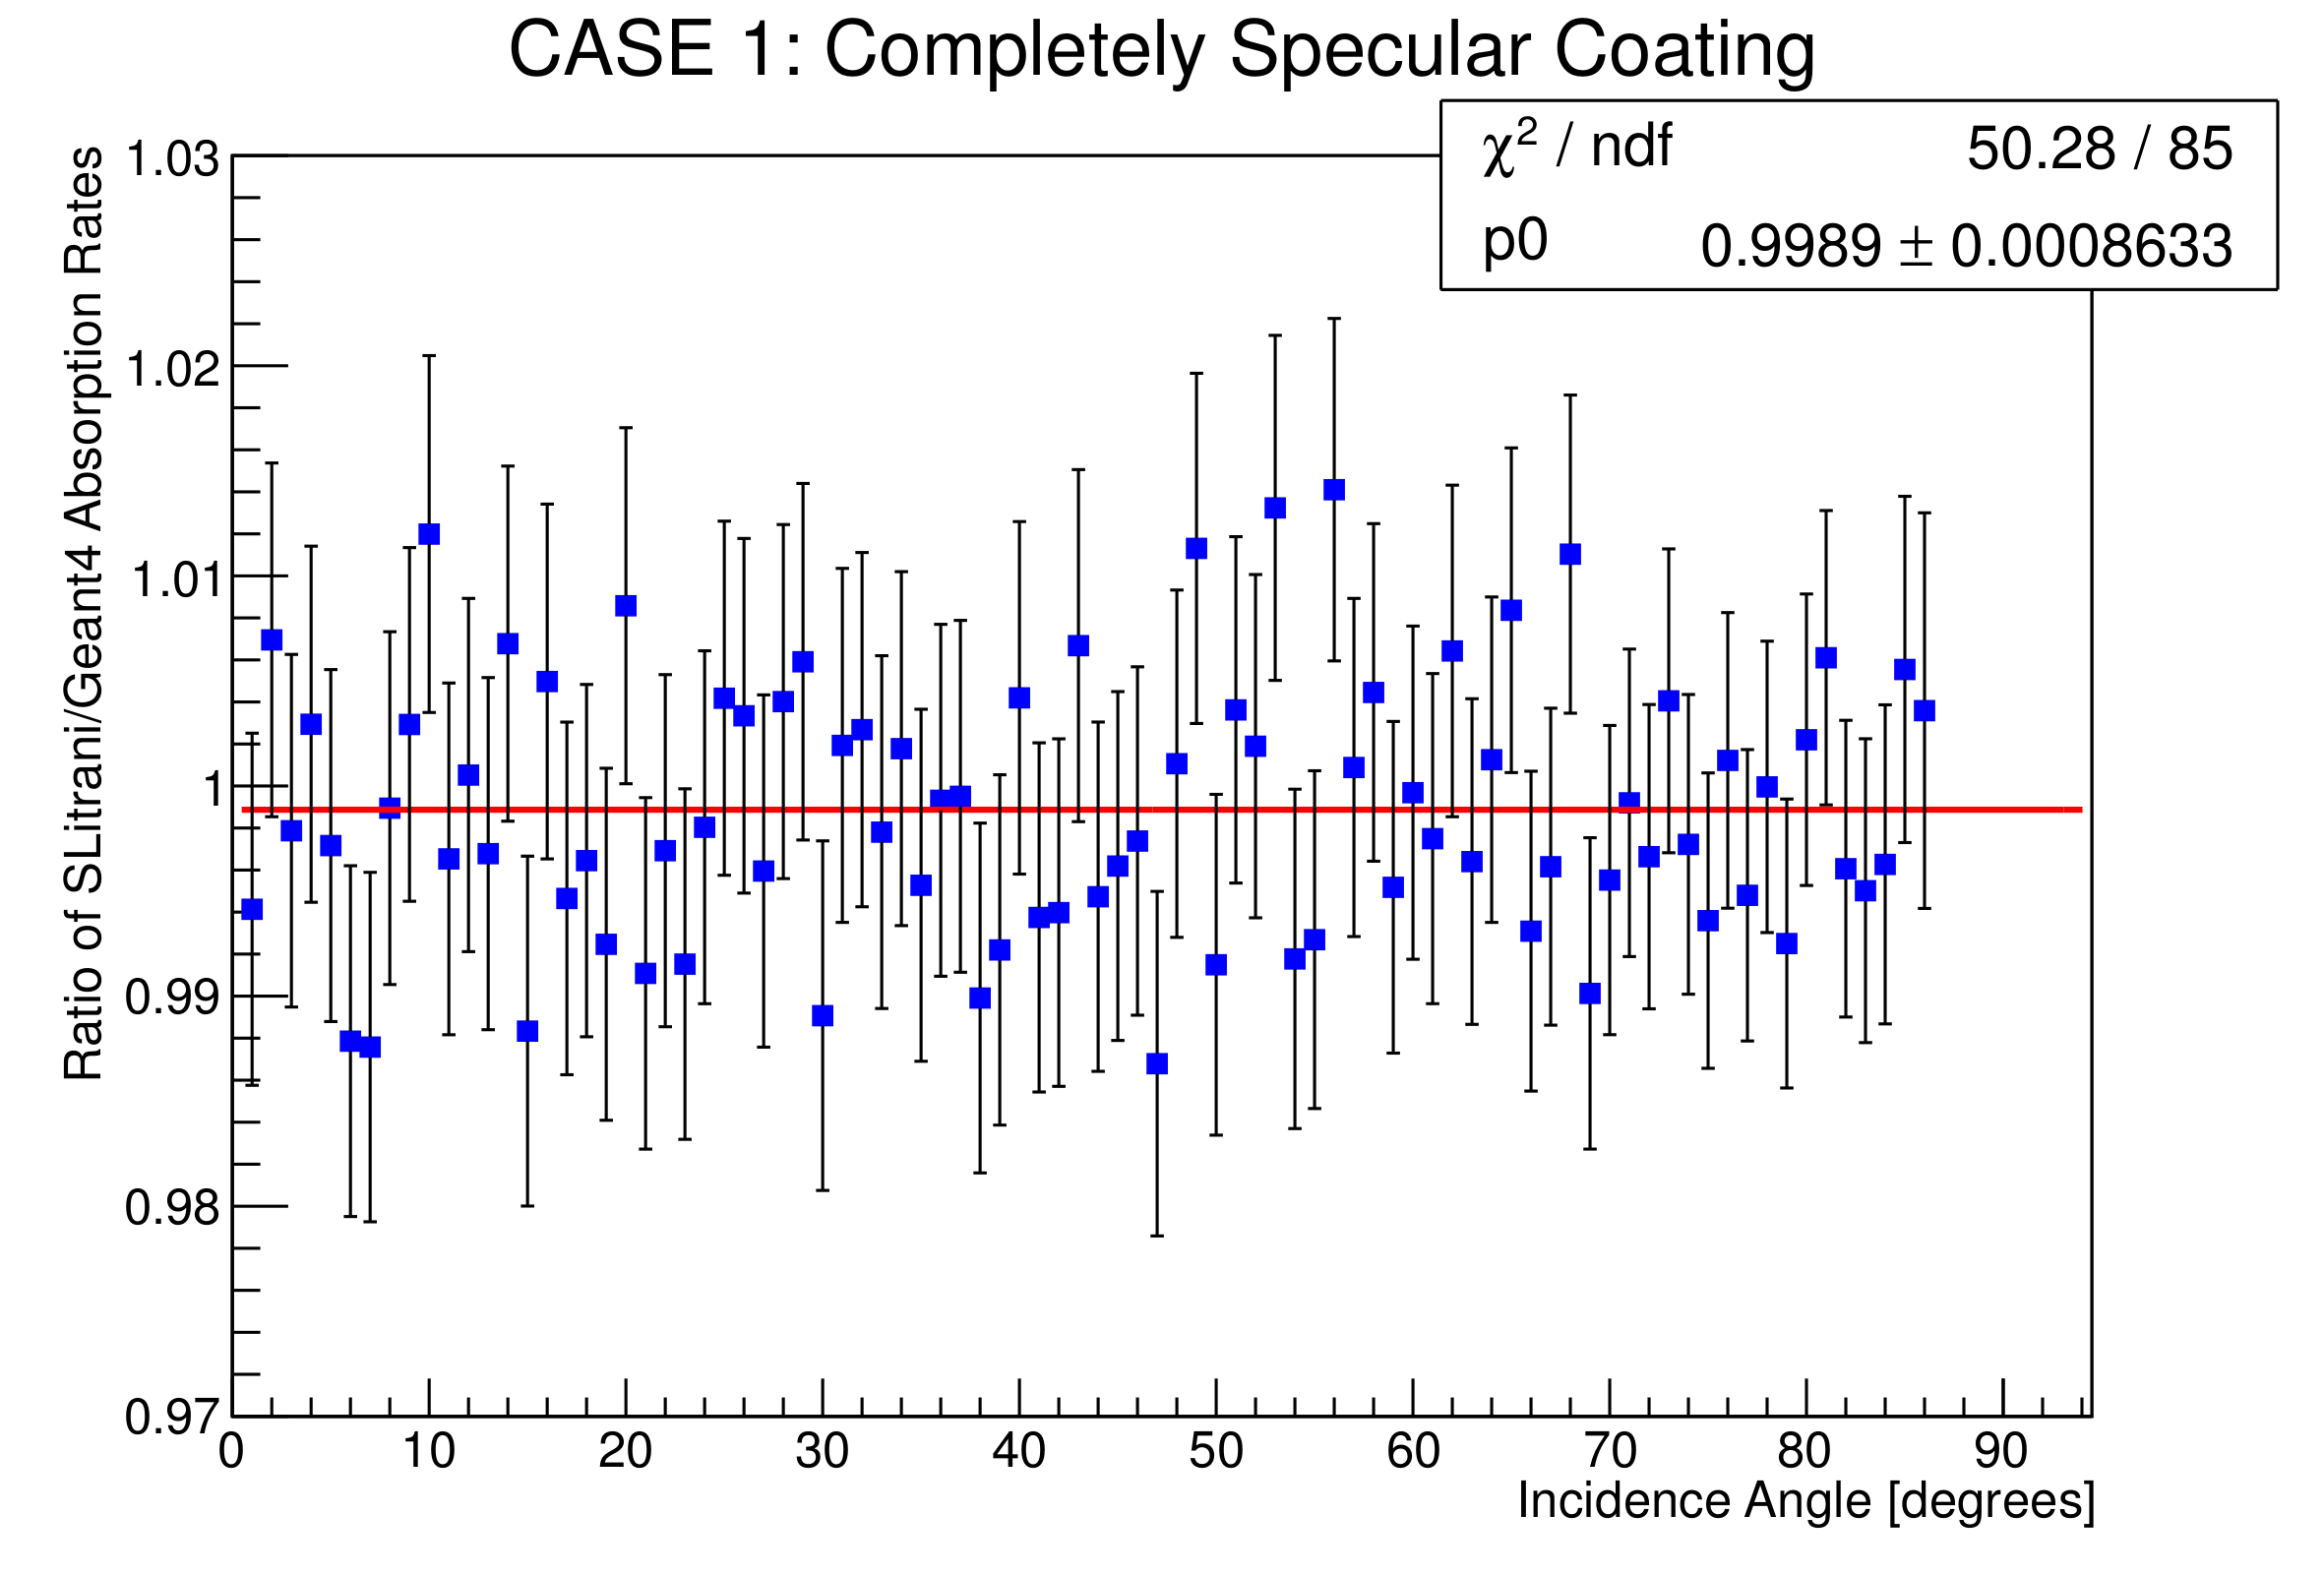
\includegraphics[width=6cm]{../Pictures/Chapter_5/specular.png}
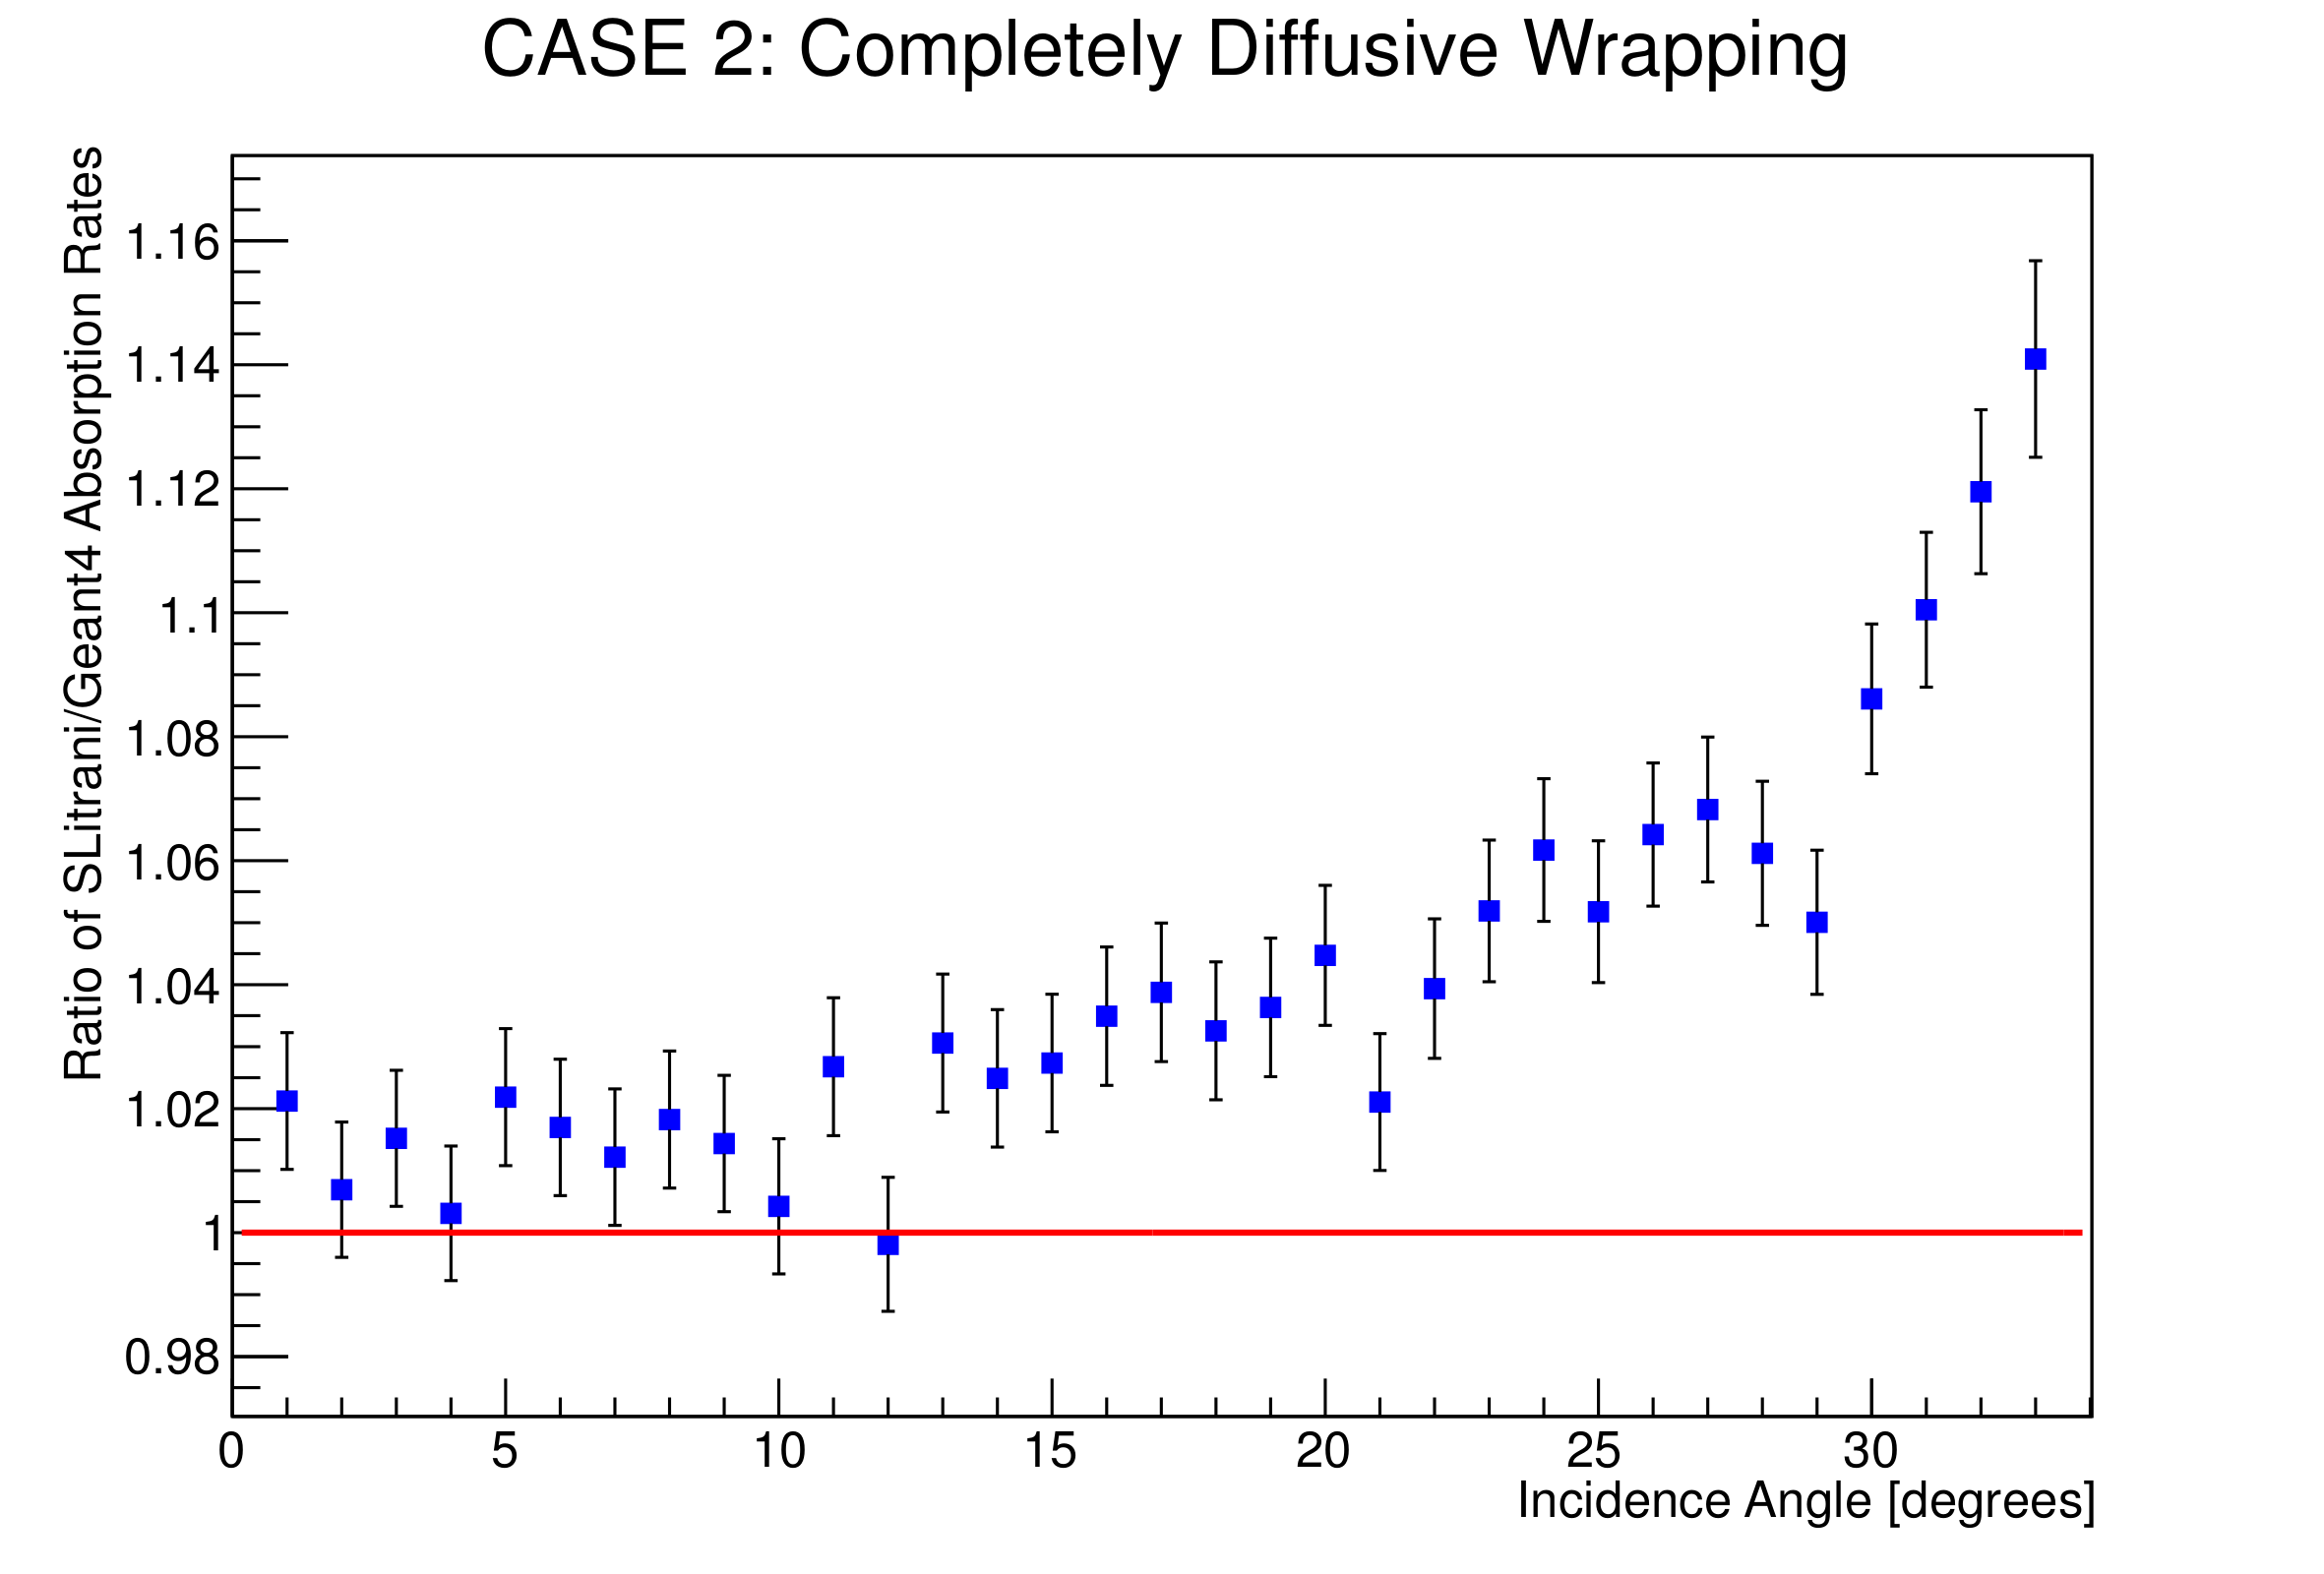
\includegraphics[width=6cm]{../Pictures/Chapter_5/diffusive.png}
\end{center}
\caption[]{}
\label{fig:surface}
\end{figure}

In order to evaluate the photon extraction efficiency in a realistic setup, a LSO crystal was simulated with an internal isotropic photon source, with a class sensor placed with air gap from on of the exit faces.
Keeping a fixed cyrstal length (20 mm) while varying transverse section (from 0.56 mm$^{2}$ to 16 cm$^{2}$), the difference in the softwares were assessed for different surface states (wrapping, coating, depolishing) and crystal coupling to the detector (air and optical grease).
The results obtained for Teflon wrapping as a completely diffusive material are shown in figure \ref{fig:dimensions}.
As already inferable form the results in figure \ref{fig:surface}, a significative difference in photon extraction efficiency is found for small crystals.
It is possible to conclude that as the crystal section decreases, more bounces on the lateral faces are necessary for extraction. As SLitrani considers a higher absorption probability on the wrapping a discrepancy is measured.
\begin{figure}[htbp]
\begin{center}
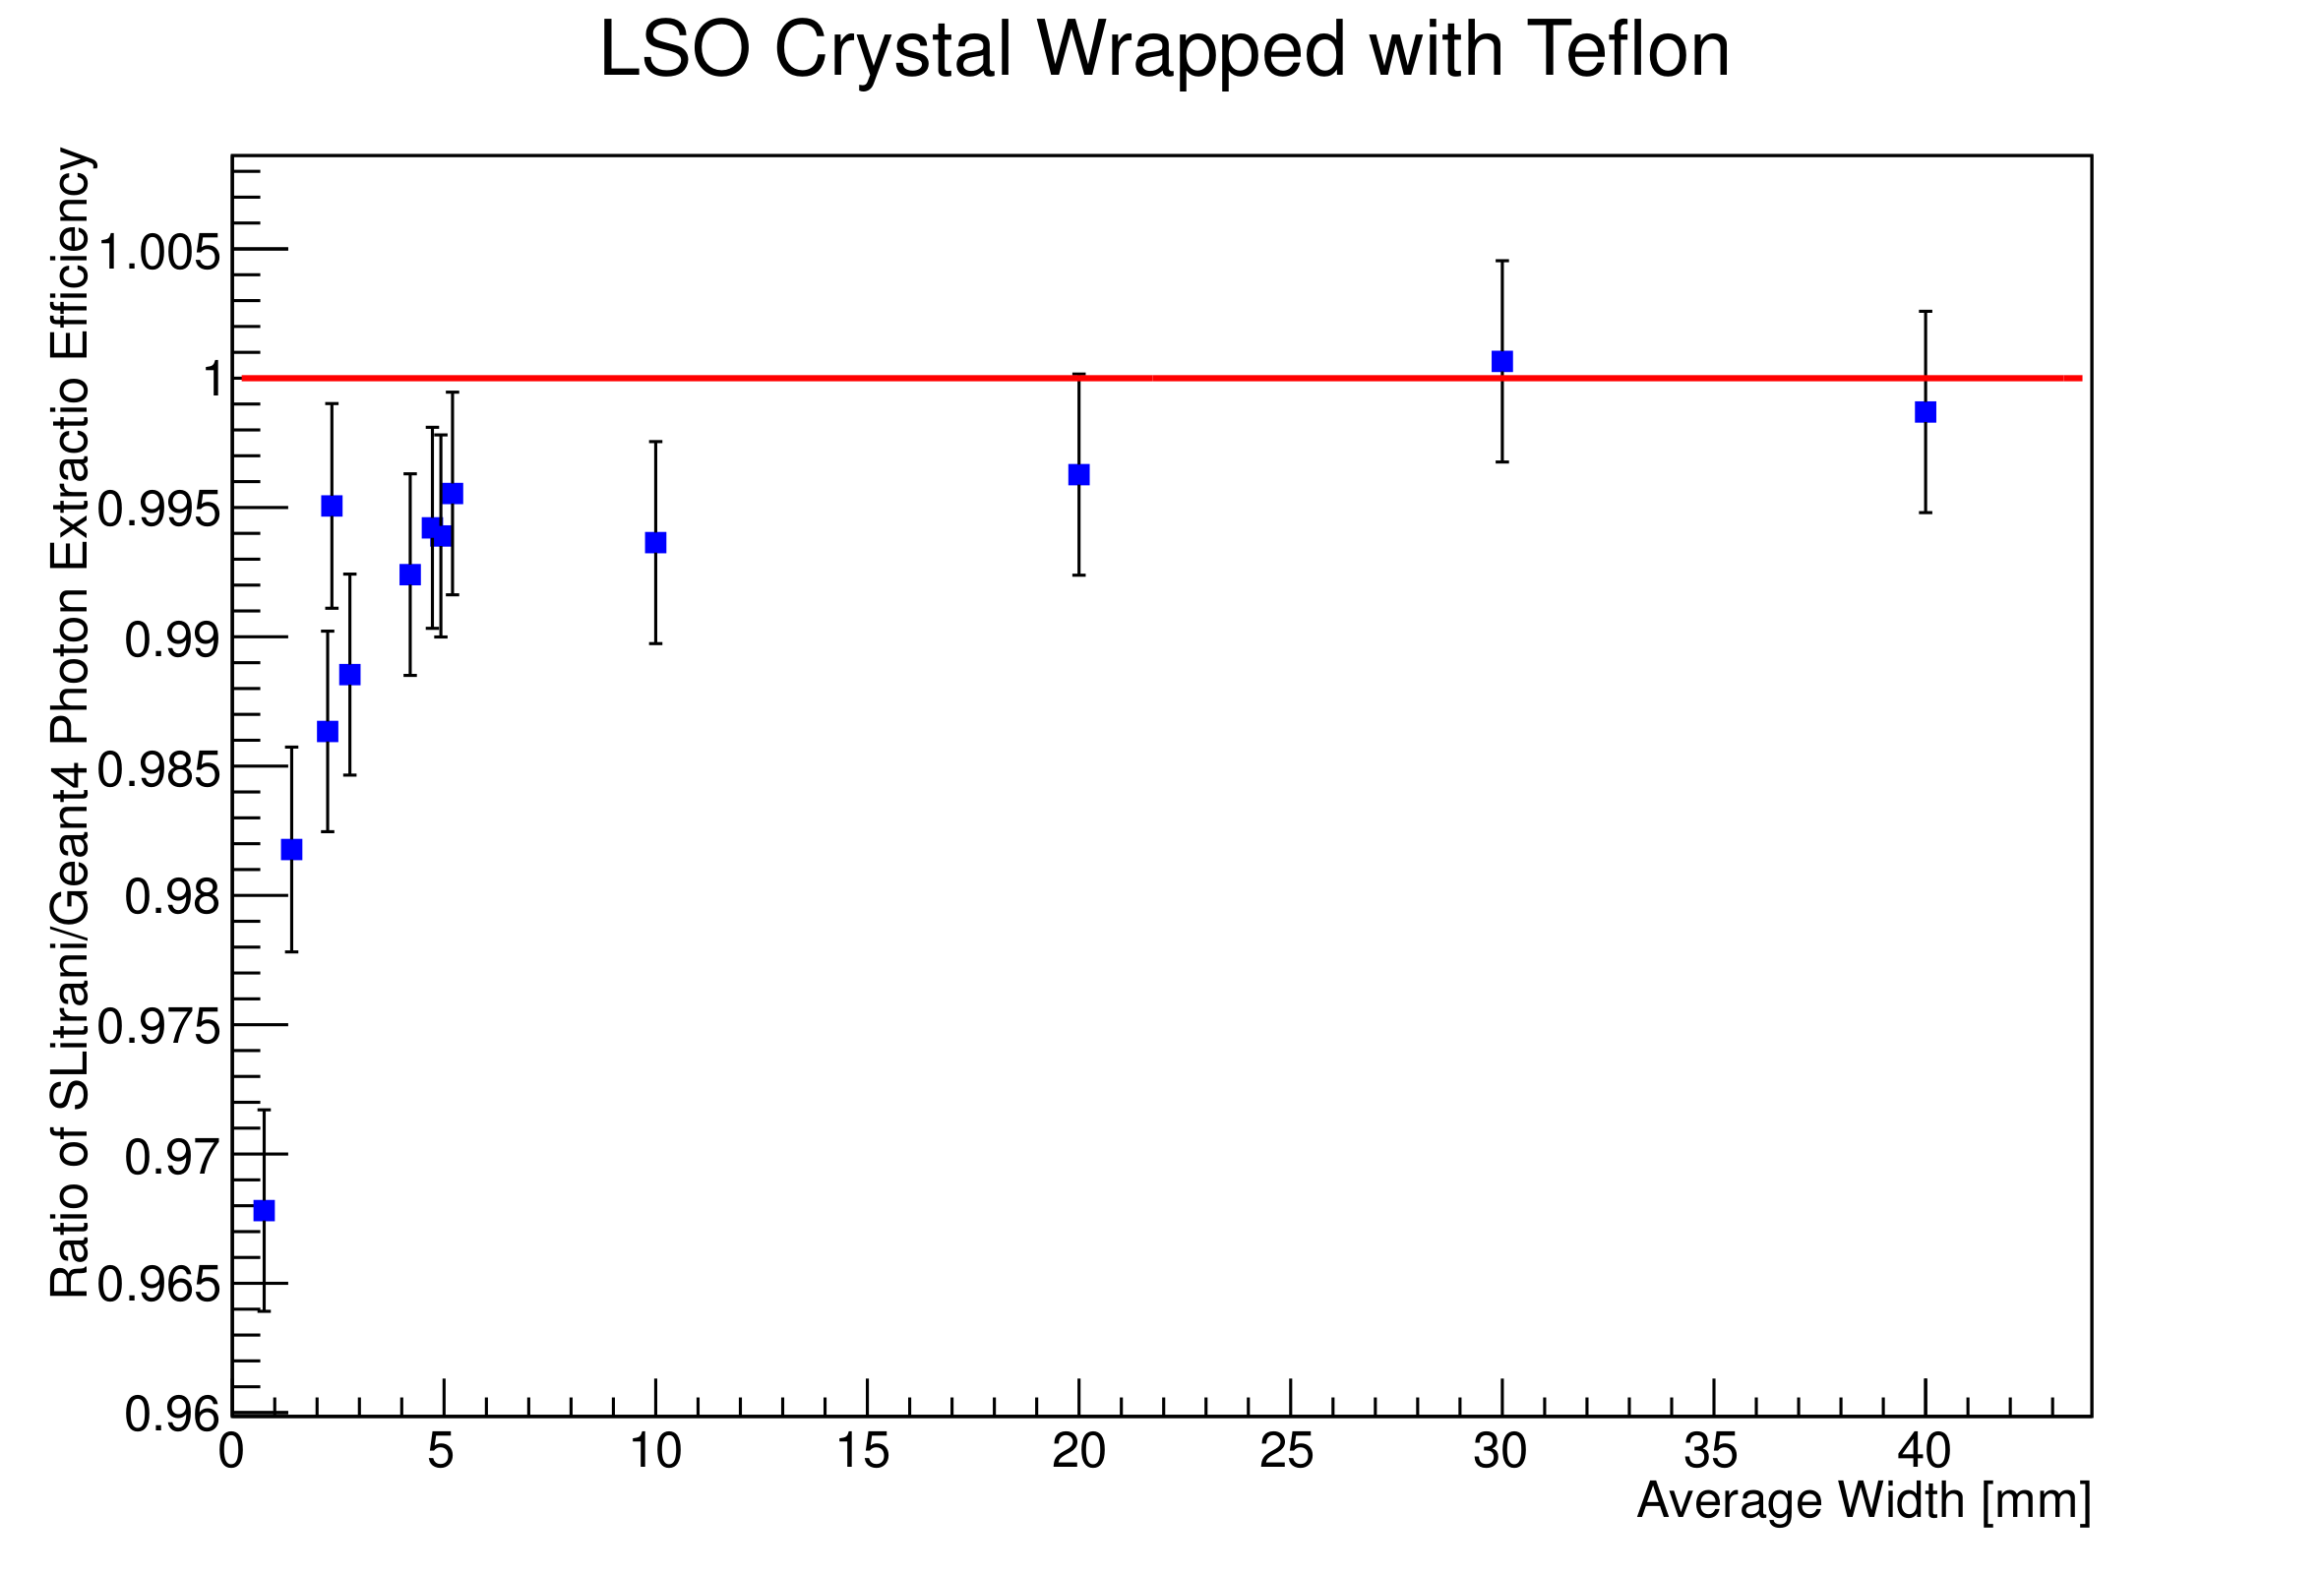
\includegraphics[width=7cm]{../Pictures/Chapter_5/size_LY_variation.png}
\end{center}
\caption[]{}
\label{fig:dimensions}
\end{figure}
This results, though, seem to back the idea that a satisfying model for boundary interaction is still lacking. In fact, as a preliminary comparison with experimental data, the values extracted in \cite{Kris2012} where considered, since full access to the experimental setup and materials was possible. 
The comparison was performed on the gain in the extraction coefficient obtained by coupling the crystal to a PMT with optical grease and by wrapping it with Teflon.
The gain given by the grease was qualitatively reproduce, as shown in figure \ref{fig:gain}. The sistematic difference is due to poor knowledge of the optical grease index of refraction. 
On the other hand, the gain due to the use of
Teflon wrapping, is significantly different between
experimental data and Monte Carlo simulations, as shown in figure \ref{fig:gain}.
\begin{figure}[htbp]
\begin{center}
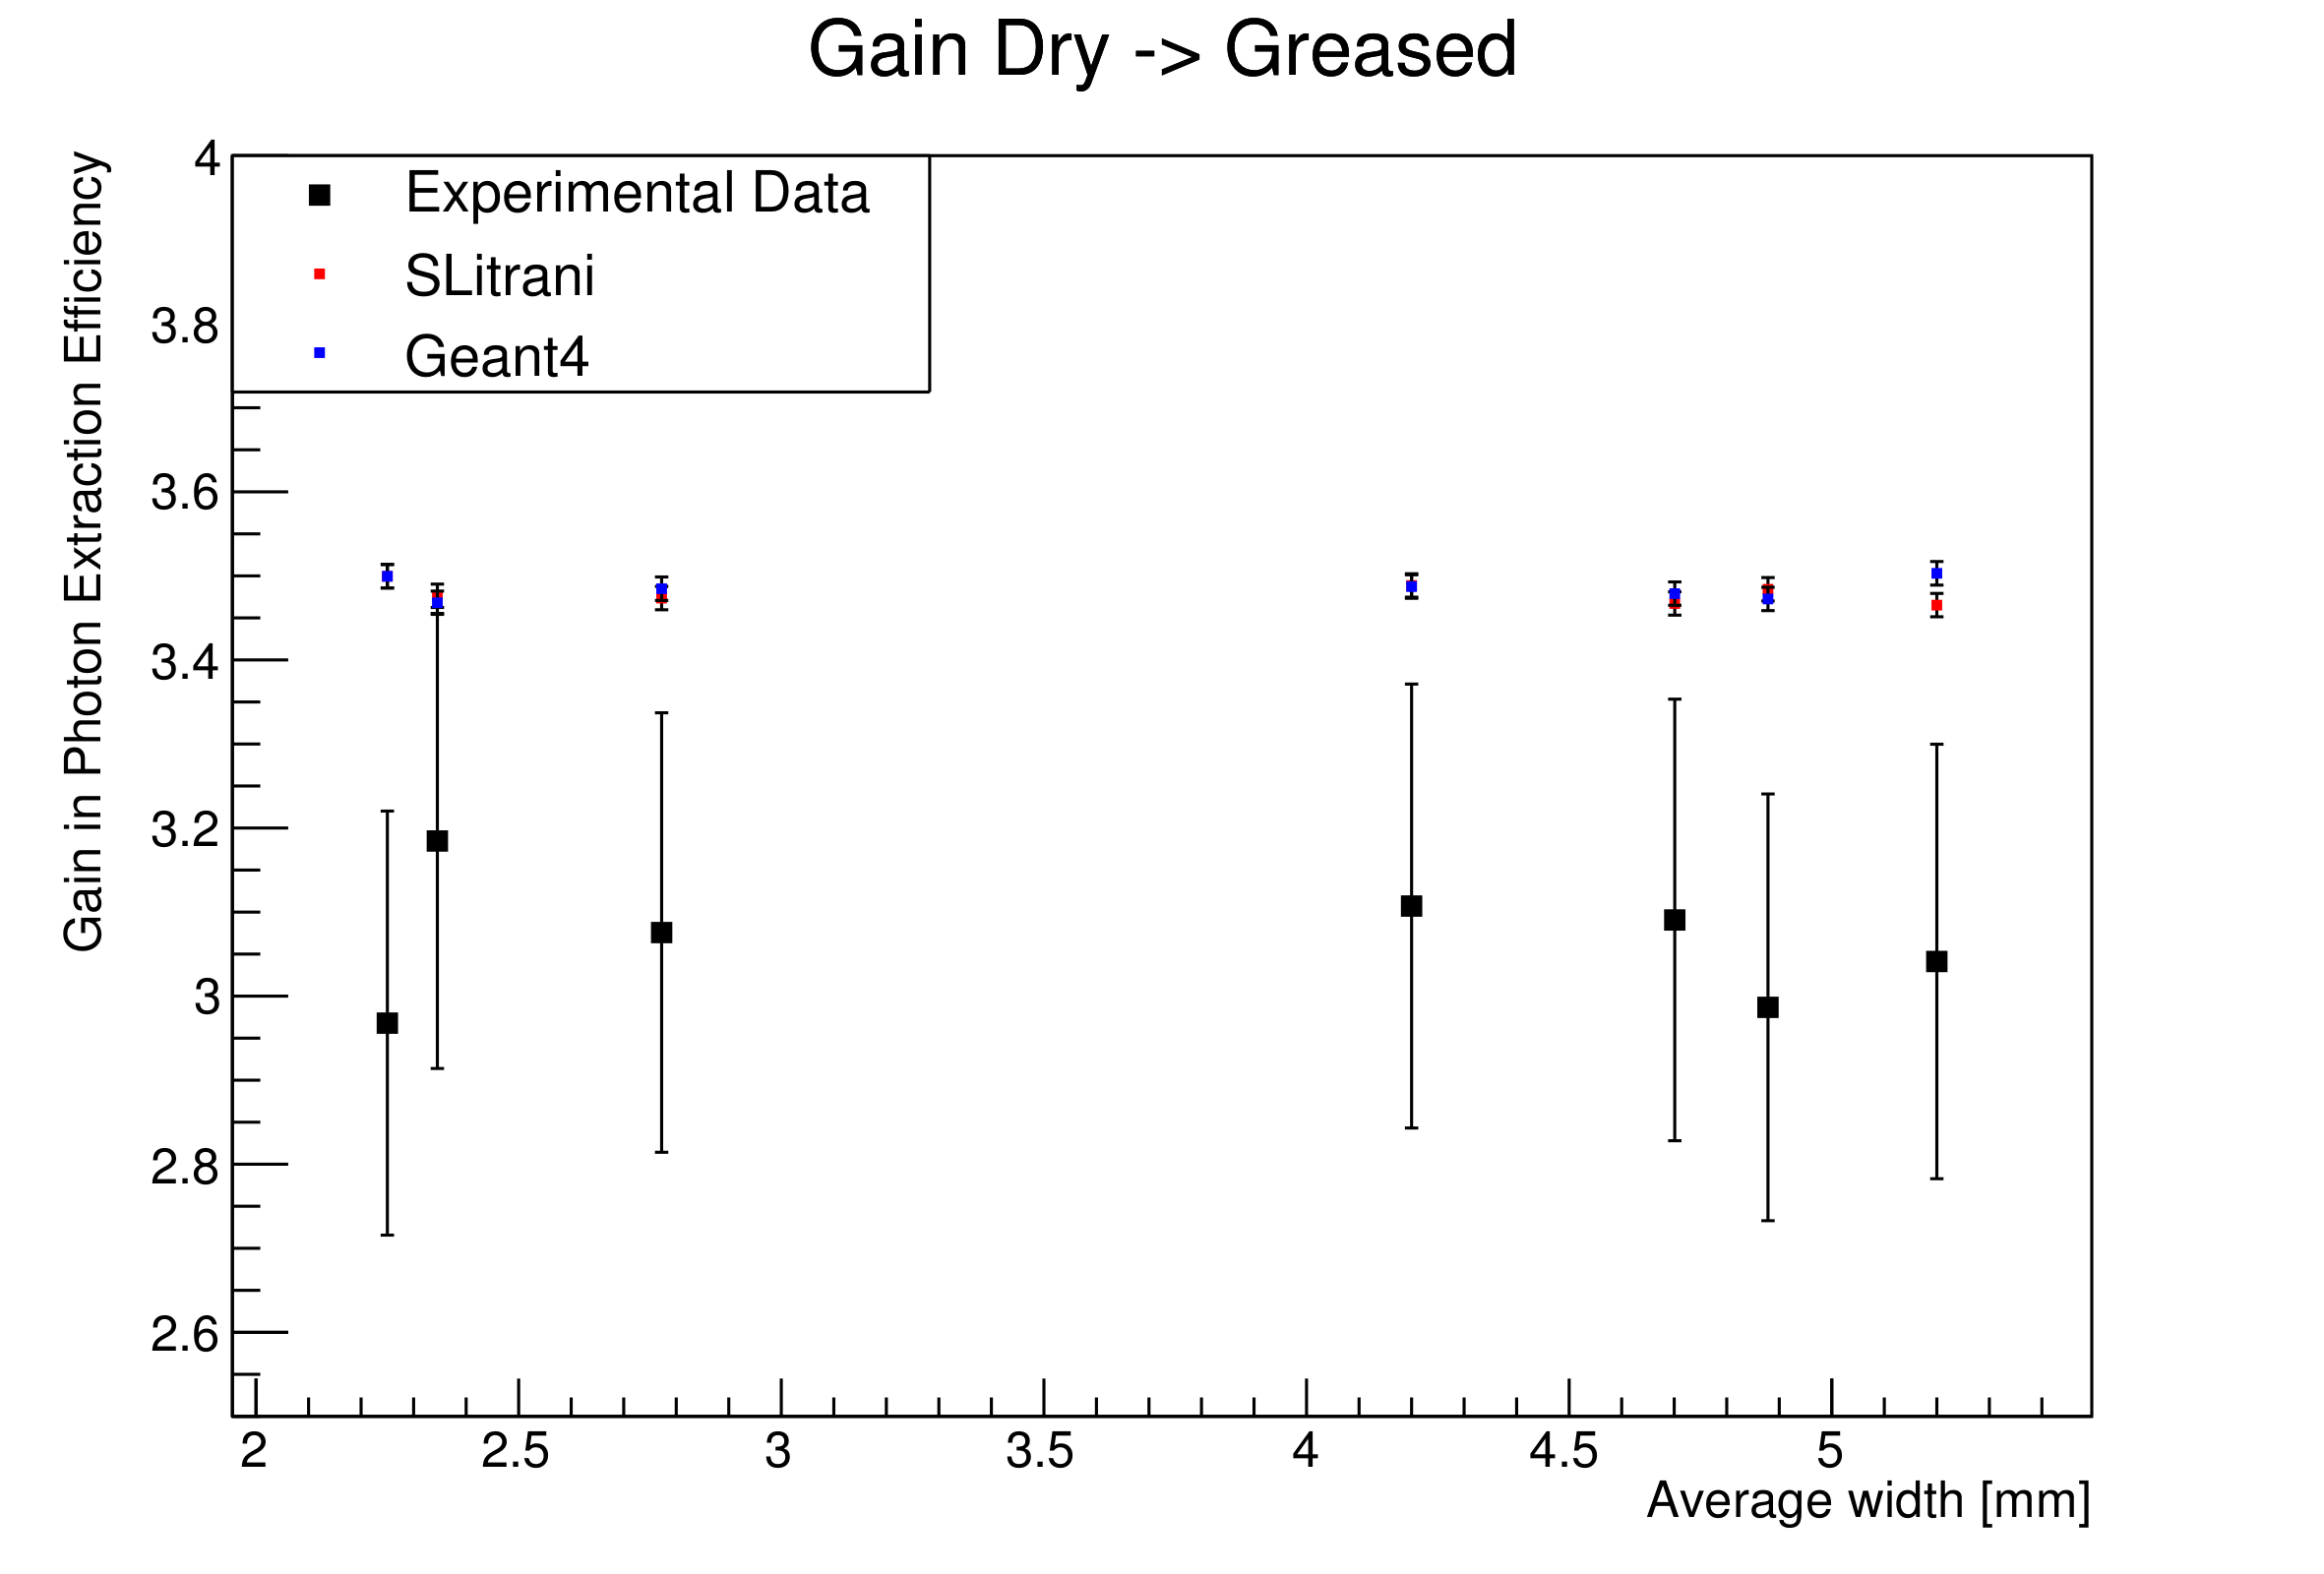
\includegraphics[width=6cm]{../Pictures/Chapter_5/gain_grease.png}
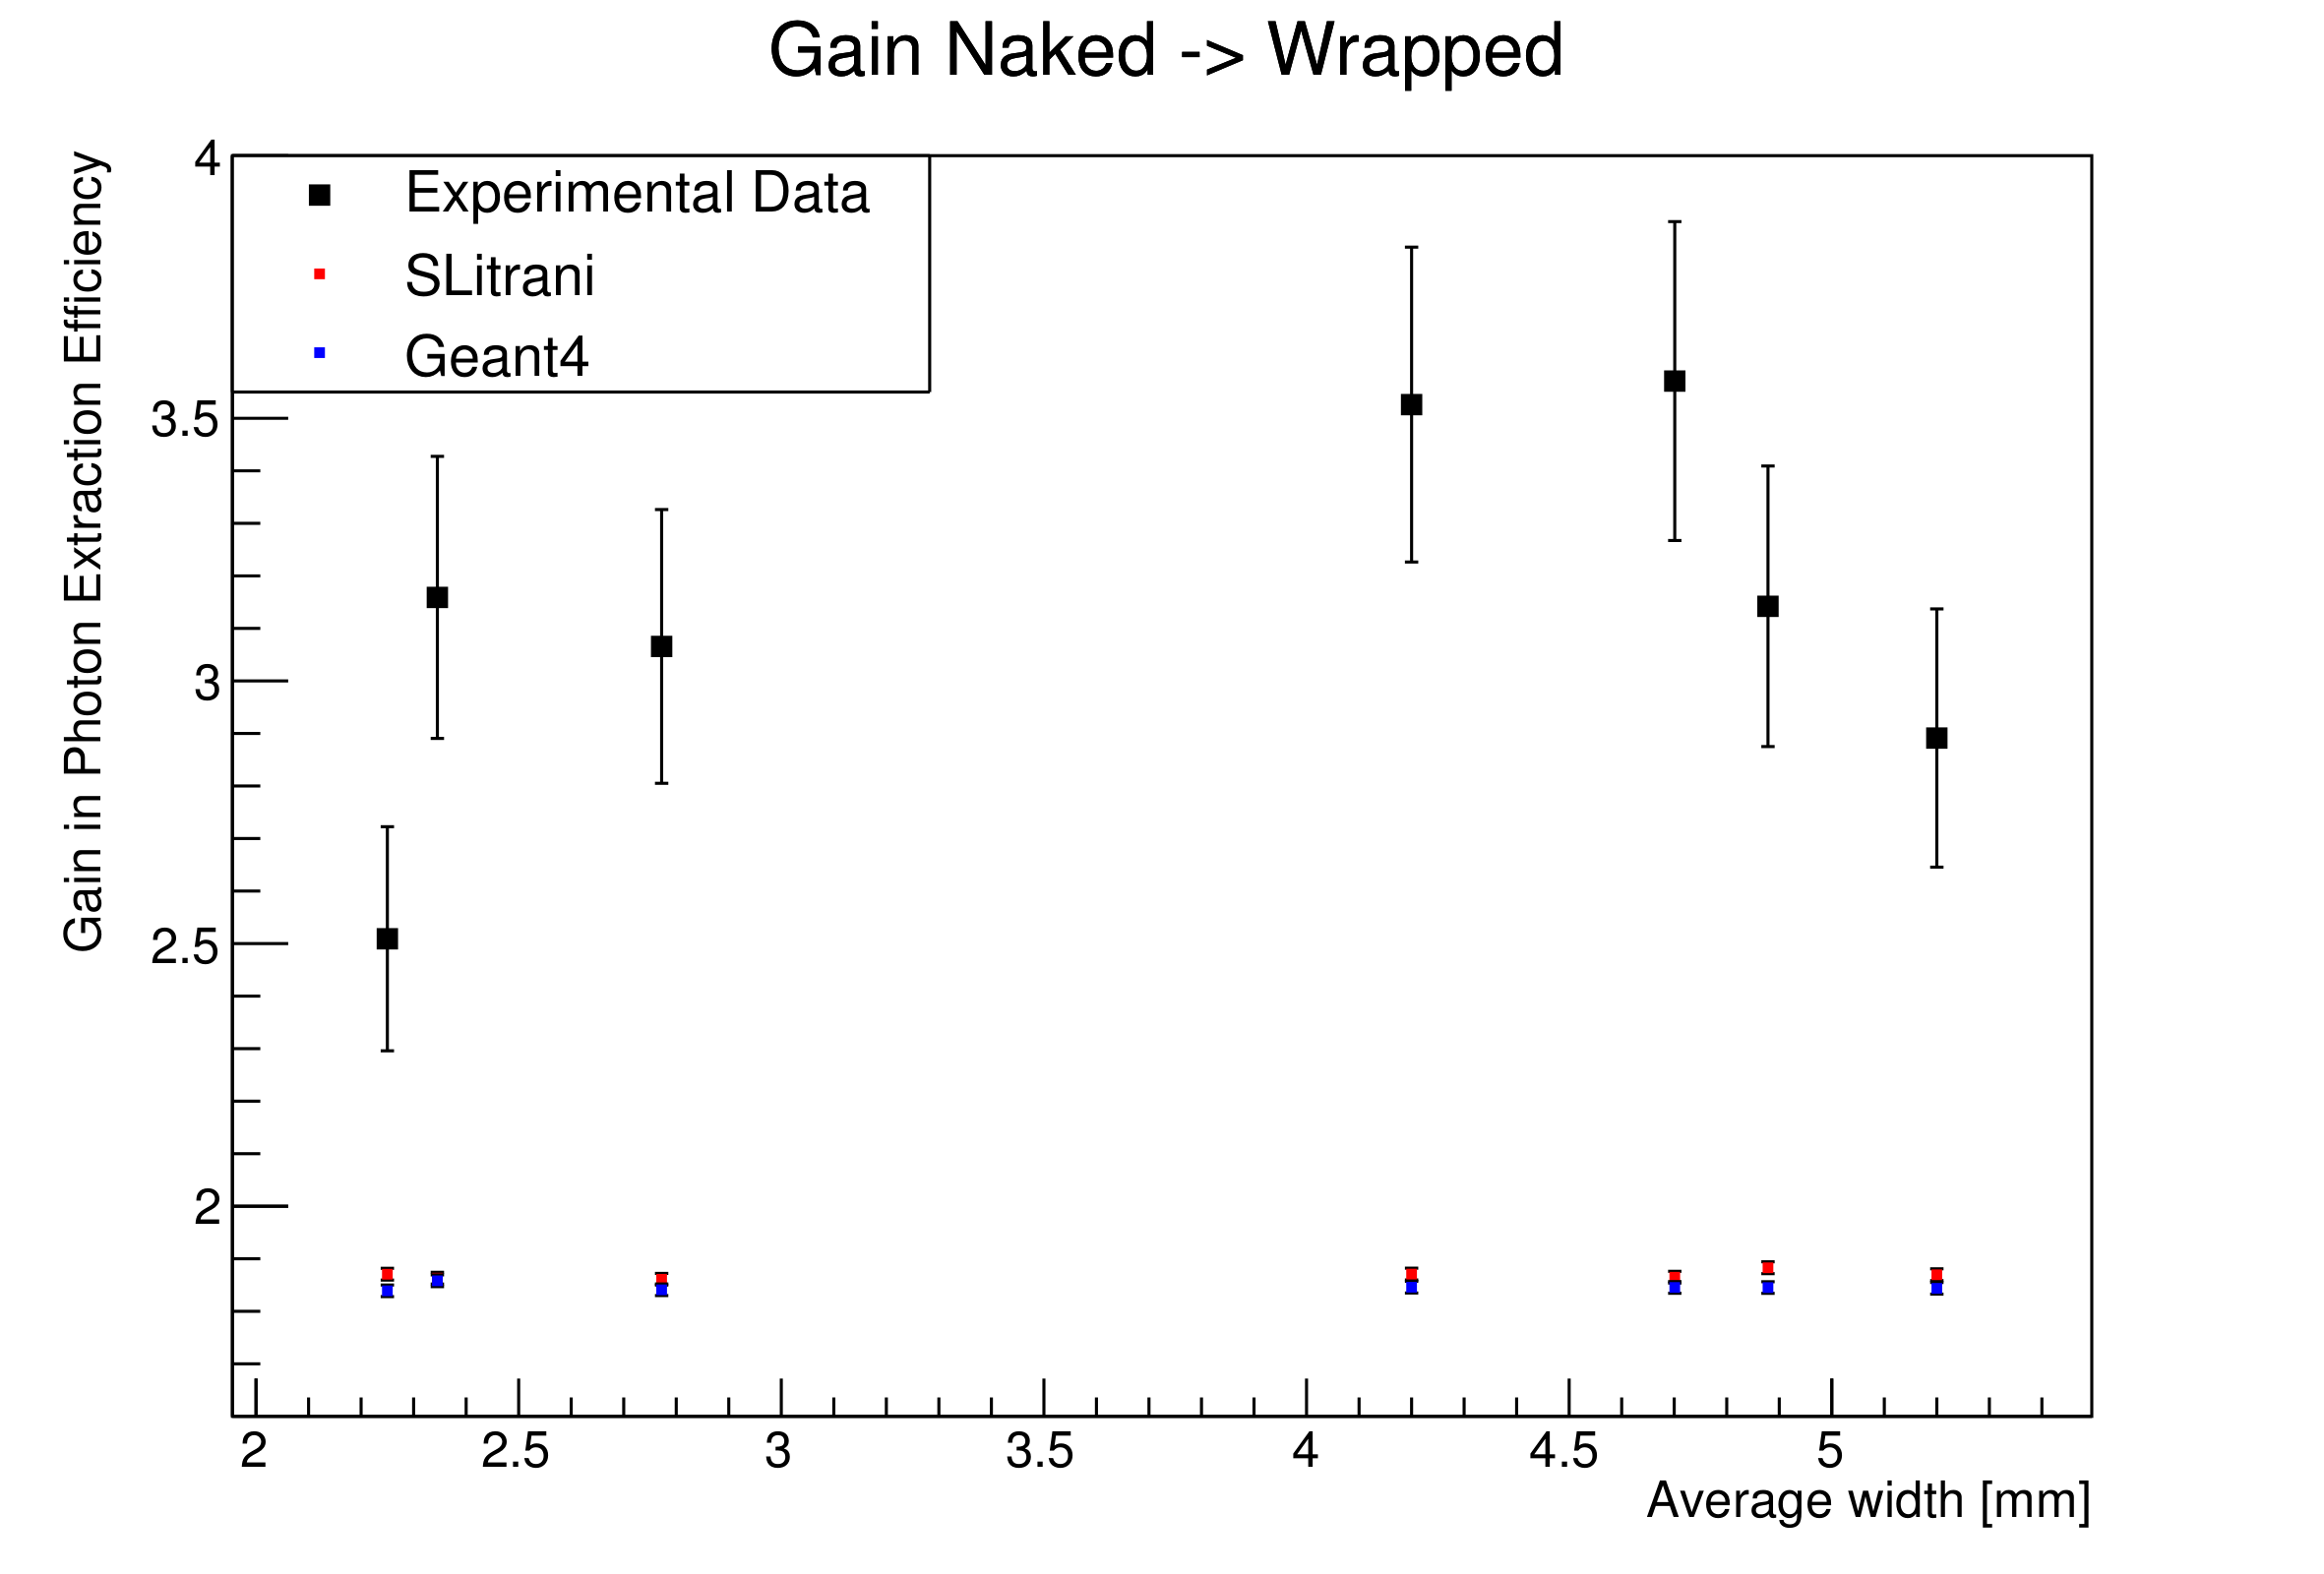
\includegraphics[width=6cm]{../Pictures/Chapter_5/wrap_gain.png}
\end{center}
\caption[]{}
\label{fig:gain}
\end{figure}
Given this poor modeling of surface interaction we relied mainly on the simplest models available for the softwares, that is polished surface and lambertian wrapping. No significative inferences can be made on light extraction, so timing simulation were tuned on parameters measured separately.
For the analysis of the measured data, we will make use of Geant4 in order to disentagle the elements contributing to signal formation in a scintillator system, since SLitrani does not offer the same processes in terms of photon production.
These three stages will be considered as the main components of the rising edge: energy deposition above the ionisation threshold, thermalization phenomena, photon coupling.

\section{Simulation input parameters}

It has emerged from the previous discussion that the time scales involved in the de excitation phases following a $\gamma$ event in a crystal, becomes relevant at the thermalization stage. This emerges also from simulation packages at the KeV scale.
After photon production optical tracking inside the volumes take place. This stage can be more and more important as the volume of the crystal grows, as scattering and absorption in the bulk, start to importantly degrade the performance of crystals in terms of light collection.
In order to properly describe this chain of processes and disentagle the various contribution that leads to the spread of the inference on the time of interaction, it is thus necessary to measure the input parameters of the crystals.
% qui l elenco va fatto bene!
For what concerns refractive indices the values previously introduced from literature were considered, since no direct method was available to measure them.
Four parameters were then accessible to experimental assessment:
\begin{itemize}
\item light yield
\item excitation spectrum
\item emission spectrum
\item transmission curve
\end{itemize}
Not all the samples were measured for Monte Carlo simulation, but only the samples whose time profiles  were characterized in the last chapter, with $\gamma$ excitation 
\begin{itemize}
\item LuAG:Ce (0.13$\%$)
\item LYSO (Sipat)
\item LYSO (Proteus)
\item LSO:Ce,Ca 
\item LSO:Ce (CTI)
\item BGO
\item CeF$_{3}$
\end{itemize}
%spiegare qui bene i sample, da richiamare rapidamente in VUV!
\subsection{Fluorescence spectrum}
In order to analyze the timing profiles of crystals measured and plug in the correct parameters for simulations, 
the energy levels of the samples were investigated with a spectro fluorimeter.
\begin{figure}[htbp]
\begin{center}
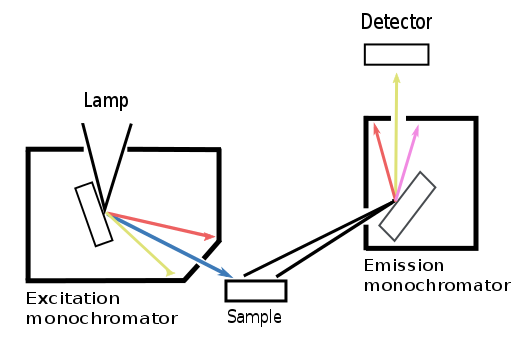
\includegraphics[width=8cm]{../Pictures/Chapter_5/fluo.png}
\end{center}
\caption[Spectro fluorimeter]{The setup used to measure excitation and emission spectra of the samples}
\label{fig:emission}
\end{figure}
 
As shown in figure \ref{fig:emission} a light source (tipically Xenon based) is used to generate photons over a certain range (200 nm - 800 nm) and two monochromators allow to select both the excitation and the emission wavelengths. 
Given a certain excitation wavelength it is then possible to measure the emission spectrum of the sample considered.
It is also possible to select a certain wavelength of emission and measure the excitation spectrum of the same sample.
Emission and excitation spectra of a LYSO (Sipat) crystal is shown in figure \ref{fig:}
The LSO, LGSO, LSO:Ce,Ca crystals do not qualitatively differ in terms of emission and excitation from the sample shown. 
Indeed the typical emission band for the 

The LuAG:Ce...

\begin{figure}[htbp]
\begin{center}
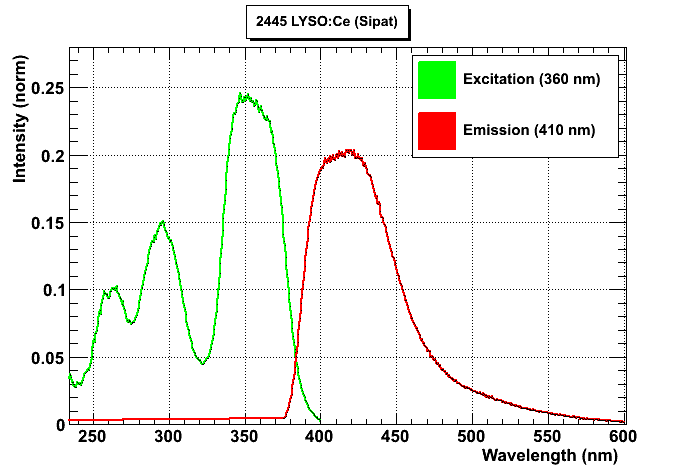
\includegraphics[width=6cm]{../Pictures/Chapter_5/LYSO_Sipat.png}
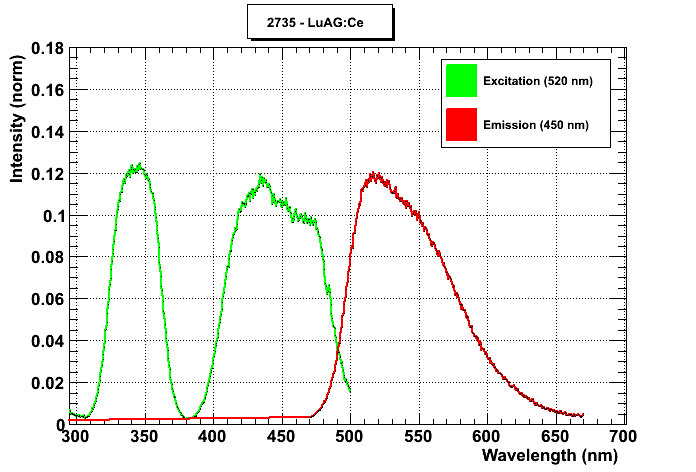
\includegraphics[width=6cm]{../Pictures/Chapter_5/LuAG_ce.png}
\end{center}
\caption[Sipat - LuAG excitation/emission]{Measured excitation and emission spectra for LYSO Sipat an LuAG: Ce}
\label{fig:luag_lso}
\end{figure}

The LuAG:Pr...

The CeF$_{3}$...

\begin{figure}[htbp]
\begin{center}
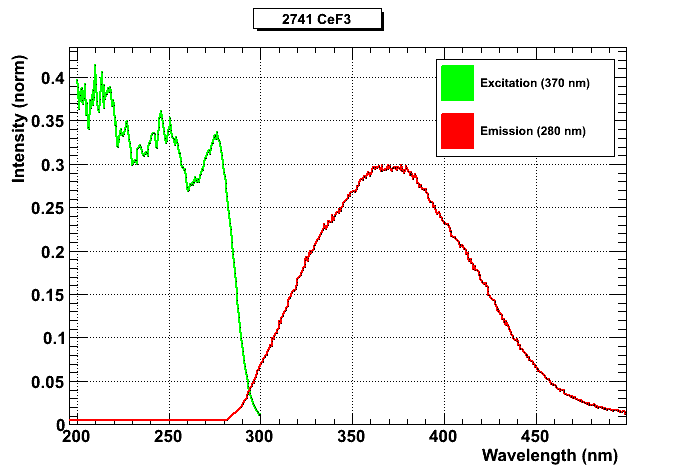
\includegraphics[width=6cm]{../Pictures/Chapter_5/cef3.png}
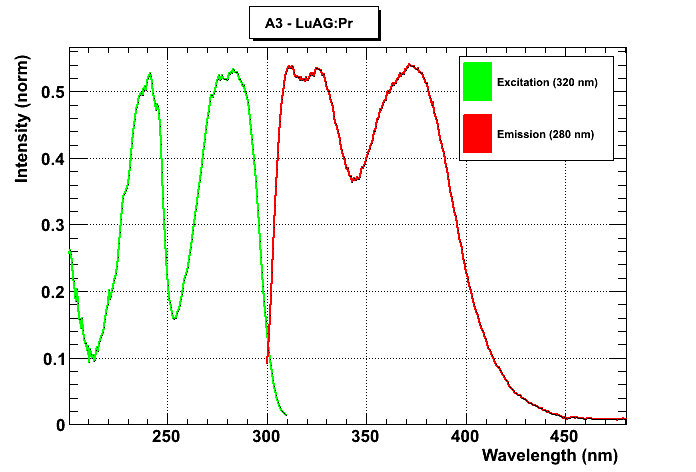
\includegraphics[width=6cm]{../Pictures/Chapter_5/LuAG_pr.png}
\end{center}
\caption[CeF$_{3}$ - LuAG excitation/emission]{Measured excitation and emission spectra for CeF$_{3}$ an LuAG: Pr}
\label{fig:luag_cef3}
\end{figure}

The BGO...

\begin{figure}[htbp]
\begin{center}
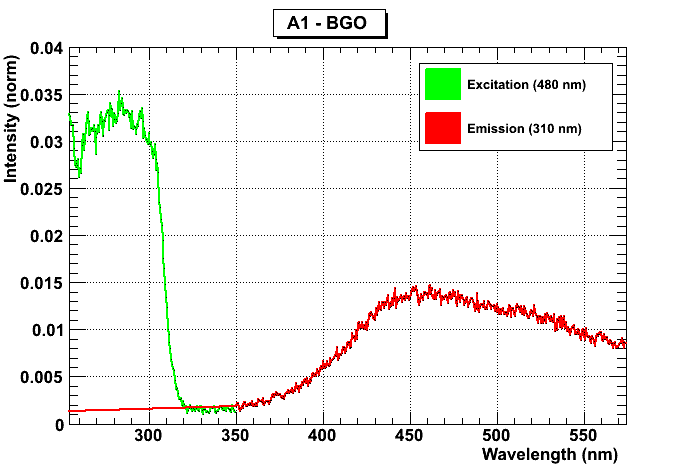
\includegraphics[width=8cm]{../Pictures/Chapter_5/BGO.png}
\end{center}
\caption[BGO excitation/emission]{Measured excitation and emission spectra for BGO}
\label{fig:BGO}
\end{figure}


\subsection{Optical transmission}
The next parameter analyzed to extract the inputs to the simulations was the light transmission of the samples measured.
In order to extract meaningful values transmission spectra were measured for samples of different size, since the error is more significative when dealing with small pixels.
\begin{figure}[htbp]
\begin{center}
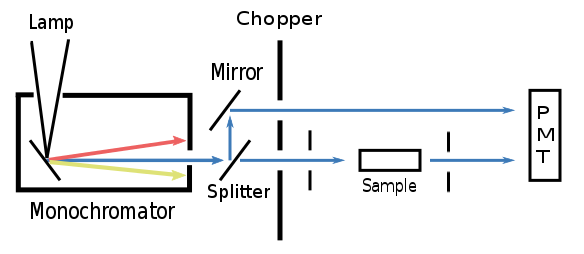
\includegraphics[width=8cm]{../Pictures/Chapter_5/trans.png}
\end{center}
\caption[Spectro photometer]{The setup used to measure the transmission curves of the samples}
\label{fig:transmission}
\end{figure}
The working principle is shown in figure \ref{fig:transmission}. The samples is crossed by a monochromatic beam of light. Before reaching the sample the beam is split, so that at the photodetector it is possible to compute the different intensities. This allows to measure the absorption length of the crystal at the different wavelengths.


\subsection{Light yield}
The definition of light yield has been already introduced in chapter 2, as well as consideration on the difference between absolute light yield and light output in a specific configuration.
Teflon tape was used as a reflector, for the case of light yield measurement as well as the $\gamma$ rise time measurement. The setup for light yield measurement is shown in figure \ref{fig:set_LY}. 
\begin{figure}[htbp]
\begin{center}
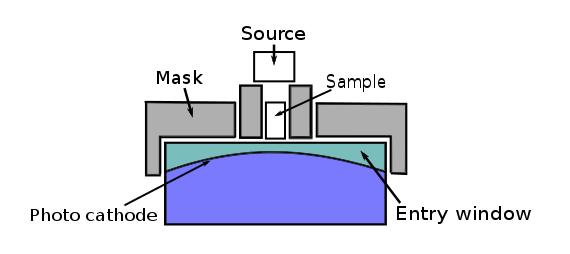
\includegraphics[width=8cm]{../Pictures/Chapter_5/LY_3.png}
\end{center}
\caption[]{}
\label{fig:set_LY}
\end{figure}
The presence of wrapping allows to couple out more photons, and in a few cases this is necessary to infer the light output (given the low intrinsic light yield), at the cost of an inferior repeatability of the measurement. The experimental error was checked with repetition of the measurement, and estimated around 5$\%$.
The light output has been measured with a $^{137}$Cs source ($E_{gamma}$ = 662 keV) placed a few millimeters above the crystal. The system crystal-PMT was placed inside a black box, with controlled temperature ($20^{\circ}C$) to avoid drift in the system response.
Further shielding against background light was ensured by an aluminum cap covering the entry window of a Hamamatsu R2059 PMT.
After the collection of the photo electrons at the anode of the PMT, the signal is attenuated, shaped and stored by the DAQ, with a digitizer \textit{CAEN DT$5720$}.

To measure the light output of sample crystals the number of photo electrons $N_{pe}$ collected can be used.
In particular by computing the area of the scintillation pulse we can obtain the number of photo-electrons collected by comparison with the value of the single electron response (SER).
The SER is measured exploiting the dark current of the PMT, caused by thermal emission of electrons from the photo cathode.
After multiplication in the dynode system, the charge integrated is the response of the PMT to a single photo electron.
The probability to emit two electrons is very low.
The number of photo electrons can be calculated by comparison with the position of the photo electric peak with respect to the signal produced by a single photon. The number of photo electron per MeV of the incident $\gamma$ particle can be determined as
\begin{equation}
N_{pe}/MeV=\frac{position\ photo\ peak}{position\ single\ photo\ electron\ peak} \cdot \frac{A_{1}}{A_{2}} \cdot \frac{1}{E_{\gamma}}
\end{equation}
where $E\gamma$ is the energy of the incident $\gamma$ particle and linearity of the detector response is assumed. A pedestal may be subtracted from the position of the peaks. $A_{1}$ and $A_{2}$ are the values of the attenuation of the signal in the case of the photo peak and the single electron peak, i.e.
\begin{equation}
A_{i}=e^{\frac{B_{i}}{20}}
\end{equation}
and $B_{i}$ is the attenuation in dB.
In order to extract the position of the photo peak and the resolution on the peak  from the charge spectra, the sum of a Gaussian and a Fermi distribution is used for the fit:
\begin{equation}
y(x)=\frac{P}{e^{\frac{x-C}{R}}+1}+Ae^{-\frac{(x-\mu)^{2}}{2\sigma ^{2}}}
\end{equation}
where P, C and 1/R correspond to height, position and slope of the Compton edge, A is the height of the photo peak with position $\mu$ and FWHM width $2.35\sigma$.
For the single photo electron spectrum a simple Gaussian fit determines the charge for the single photon with sufficient accuracy, at 1.6 pC.
An example of the light yield spectrum the single photo electron spectrum are shown in figure \ref{fig:spectrum}.
\begin{figure}[htbp]
\begin{center}
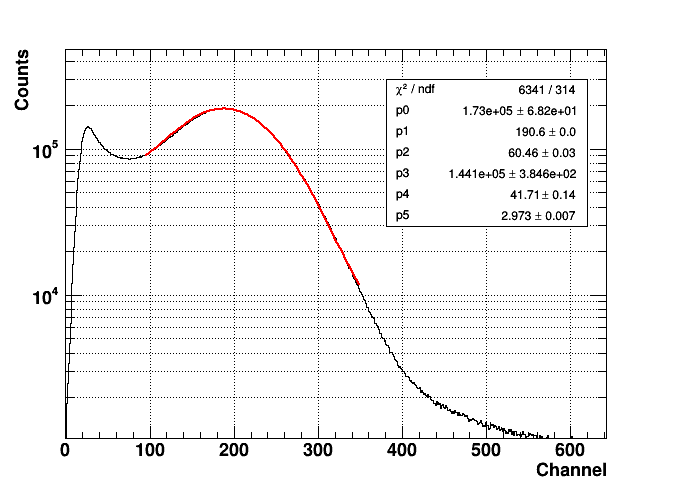
\includegraphics[width=6cm]{../Pictures/Chapter_5/single.png}
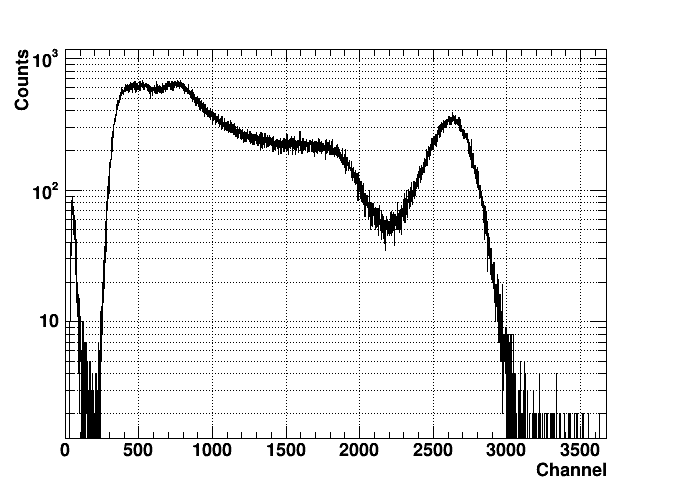
\includegraphics[width=6cm]{../Pictures/Chapter_5/spectrum_LY.png}
\end{center}
\caption[]{}
\label{fig:spectrum}
\end{figure}
At this point the number of photons extracted per MeV can be determined if the quantum efficiency of the photo detector is known:
\begin{equation}
N_{ph}/MeV=\frac{N_{pe}}{QE}
\end{equation}
In order to determine the average quantum efficiency given a certain sample, the emission curve of the sample itself was used, and weighted by the quantum efficiency curve of the PMT (shown in figure \ref{fig:QE}.
Finally the integration time was optimised on the time profile of the crystal measured, so that for LSO was set to 400 ns and for LuAG to 4 $\mu$s.
\begin{figure}[htbp]
\begin{center}
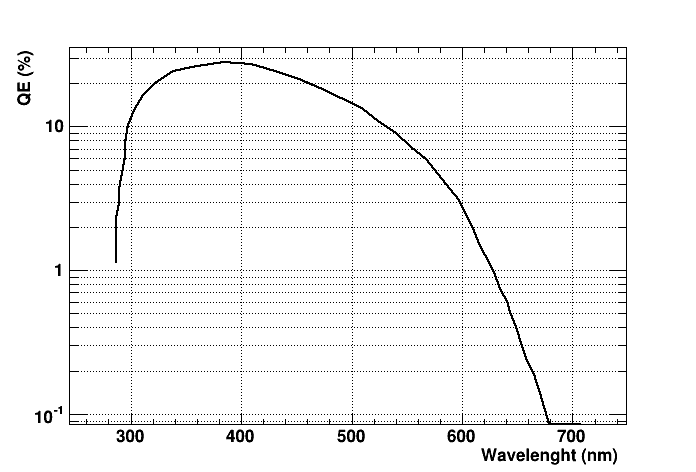
\includegraphics[width=7cm]{../Pictures/Chapter_5/qe.png}
\end{center}
\caption[]{}
\label{fig:QE}
\end{figure}
To correct for long-term variations of the PMT gain and quantum efficiency, the light output of a reference crystal is used. In order to guarantee repeatability the crystal is encapsulated into Teflon to protect it. The sample is a is $2\times 2\times 10$ $mm^{3}$ LuAP crystal.
The samples measured and relative size are shown in table \ref{table:LYtable} along with the result obtained are shown in table. Some crystals present such a low light output that it was not possible to infer the photopeak position in a naked configuration. The only available data point is with Teflon wrapping.
% come lo determino? da vedere!
\begin{table}[h]
\begin{center}
\begin{tabular}{llllll}
Crystal  & L0 (Teflon) & Res (Teflon) & LO (naked) &  Res(naked) & QE\\
LSO:Ce,Ca& 8536&15 & 3456&16 &0.22\\
LYSO:Ce (Sipat)&11002 &15 &4814 &16&0.22\\
LYSO:Ce (Proteus)& 13879& 12.9 & 4692& 17.3&0.22\\
LSO:Ce (CTI)&15583 &11.9 &5200 &14&0.22\\
LGSO:Ce & 10255&13.7 &3934 &14.1&0.22\\
CeF$_{3}$2300&26 & & & &0.22\\
LuAG:Ce (0.13$\%$)& & & & &0.1\\
BGO& & & & &0.16
\end{tabular}
\end{center}
\label{table:LYtable}
\end{table}

